\pdfminorversion=4
\documentclass[xcolor=dvipsnames,hyperref={pdfpagelabels=false},unknownkeysallowed]{beamer}
\usepackage{tabls}
\usepackage{picture}
\usepackage{graphicx}
\usepackage{tcolorbox}
\usepackage{subcaption}
\captionsetup{compatibility=false}
%\usepackage{animate}

%To add a grid to the slides for aligning stuff
%\usepackage[texcoord,grid,gridunit=mm,gridcolor=gray,subgridcolor=gray!10,gridBG=true]{eso-pic}



%Tikz stuff
\usepackage{tikz}
\usetikzlibrary{shapes.geometric, arrows,shapes.arrows,calc,positioning}
\tikzstyle{startstop} = [rectangle, rounded corners, minimum width=2cm, text
    width=1.8cm, minimum height=1cm,text centered, text=white,draw=black, fill=Gray!140]
\tikzstyle{io} = [trapezium, trapezium left angle=70, trapezium right angle=110,
minimum width=0.5cm, minimum height=1cm, text centered, draw=black,
fill=blue!20!Gray!90!,text=white]
\tikzstyle{process} = [rectangle, minimum width=2cm, minimum height=1cm, text
centered, text width=2cm, draw=black, text=white,fill=Gray!140!blue!70!white]
\tikzstyle{decision} = [diamond, minimum width=2.0cm, minimum
    height=0.81cm,aspect=1.40, text centered, draw=black, fill=Gray!,text=white]
\tikzstyle{arrow} = [thick,line width=0.5mm,->,>=stealth]
\tikzstyle{arrow1} = [dashed,->,>=stealth]


\tikzset{>=stealth}

\newcommand{\tikzmark}[3][]{\tikz[overlay,remember picture,baseline] \node [anchor=base,#1](#2) {\ensuremath{#3}};}







\usepackage[absolute,overlay]{textpos}

\newdimen\pc \pc=14bp
\def\XY#1#2{\xy{#1\pc}{#2\pc}}

\newcommand\myblock[3]{%
    \begin{textblock*}{\paperwidth}(#1\paperwidth,#2\paperwidth)
        \raggedright #3\hspace{0.5em}
    \end{textblock*}}



\definecolor{myblue}{rgb}{0.7, 0.7, 60.0}
\definecolor{mylightblue}{rgb}{1,1,1}
\newcommand*{\boxedcolor}{blue}
\makeatletter
\renewcommand{\boxed}[1]{\textcolor{\boxedcolor}{%
  \fbox{\normalcolor\m@th$\displaystyle#1$}}}
\makeatother

\newcommand{\highlight}[1]{%
    \colorbox{myblue!50}{\ensuremath{\displaystyle#1}}}

\renewcommand{\u}[1]{\underline{#1}}

\newcommand{\iso}[2]{${}^{{#2}}${#1} }
\newcommand{\nubar}[0]{\ensuremath{\overline{\nu}} }
\newcommand{\keff}[0]{\ensuremath{{k}_{\textsf{eff}}} }
\newcommand{\sa}[0]{\ensuremath{\sigma_c} }
\newcommand{\sfiss}[0]{\ensuremath{\sigma_f} }
\newcommand{\st}[0]{\ensuremath{\sigma_t} }
\newcommand{\ds}[0]{\displaystyle}
\newcommand{\expect}[1]{E[#1] }
\newcommand{\colg}[1]{{\color{ForestGreen} #1}}
\newcommand{\coly}[1]{{\color{yellow} #1}}
\newcommand{\colb}[1]{{\color{blue} #1}}
\newcommand{\colG}[1]{{\color{Gray!110} #1}}
\newcommand{\colr}[1]{{\color{red} #1}}
\usepackage{amsfonts}
\newlength{\wideitemsep}
\newlength{\tabsep}
\setlength{\tabsep}{0.99cm}
\setlength{\wideitemsep}{8pt}
\addtolength{\wideitemsep}{5pt}
\let\olditem\item
\renewcommand{\item}{\setlength{\itemsep}{\wideitemsep}\olditem}

\newcommand{\N}{\mathbb{N}}
\newcommand{\Z}{\mathbb{Z}}
\newcommand{\deriv}[2]{\frac{\mathrm{d} #1}{\mathrm{d} #2}}
\newcommand{\pderiv}[2]{\frac{\partial #1}{\partial #2}}
\newcommand{\bx}{\mathbf{X}}
\newcommand{\ba}{\mathbf{A}}
\newcommand{\by}{\mathbf{Y}}
\newcommand{\bj}{\mathbf{J}}
\newcommand{\bs}{\mathbf{s}}
\newcommand{\B}[1]{\ensuremath{\mathbf{#1}}}
\newcommand{\Dt}{\Delta t}
\renewcommand{\d}{\mathsf{d}}
\newcommand{\mom}[1]{\langle #1 \rangle}
\newcommand{\cur}[1]{\left\{ #1 \right\}}
\newcommand{\xl}{{x_{i-1/2}}}
\newcommand{\xr}{{x_{i+1/2}}}
\newcommand{\il}{{i-1/2}}
\newcommand{\ir}{{i+1/2}}
\newcommand{\shorttitle}{\color{black} A HOLO Algorithm for Thermal Radiative Transfer
    \makebox[\linewidth]{\rule{\textwidth}{5pt}}
}

%The next lines automatically add outline slides at start of each section
\AtBeginSection[]
{
    \begin{frame}<*>
        \frametitle{\shorttitle}
        \vspace{0pt}
        \begin{minipage}[c][0.6\textheight]{0.2\textwidth}
            \hspace{-2em}
\includegraphics[width=\textwidth]{tamu_seal.png}\hspace{1em}
            \rule[-0.3\textheight]{1pt}{0.8\textheight}
        \end{minipage}
    \vspace{0pt}
        \begin{minipage}[c][0.6\textheight]{0.74\textwidth}
        \tableofcontents[currentsection,currentsubsection]
         \end{minipage}
    \end{frame}
}

\setbeamerfont{frametitle}{size=\fontsize{13.7pt}{14.2pt}}
\setbeamerfont{normal font}{size=\tiny}

\graphicspath{{figures/}}

\usepackage{verbatim}
\usepackage{comment}
\usepackage[]{datetime}
\usepackage{multirow}
\newcommand{\thedate}{\today}

%Adjust margin to be more towards the right
\setlength\leftmargini{0.17\textwidth}
\addtolength\leftmarginii{0.05\textwidth}
\setbeamersize{sidebar width left=0.21em}
\setbeamersize{sidebar width right=0.21em}
\addtobeamertemplate{frametitle}{\vspace{0.31em}}{}

%\addtobeamertemplate{navigation symbols}{}{ %
%    \usebeamerfont{footline}%
%    \usebeamercolor[fg]{footline}%
%    \insertframenumber/\inserttotalframenumber
%}


% HACKING IN page numbers
%
%    \expandafter\def\expandafter\insertlogo\expandafter{%
%        \insertlogo\hspace{4pt}%
%        \raisebox{-6.9pt}{\scriptsize{\insertframenumber\,/\,\inserttotalframenumber}}}

\setlength{\tabcolsep}{1.05cm}

%Aggie-themed
\pgfdeclareimage[height=0.1in]{TAMUlogo}{tamu_engineering.png}
%\logo{\raisebox{-8pt}{\pgfuseimage{TAMUlogo}}}
\setlength\tabcolsep{0.2310in}
\titlegraphic{\centering\begin{tabular}{lcr}\hspace{-2em}
\includegraphics[trim=0.0in 0.0in 0.0in 0.0in,clip,height=0.18\textheight]{NEUP.jpg} &
 \hspace{-1em}
\includegraphics[height=0.18\textheight]{tamu_seal.png} &
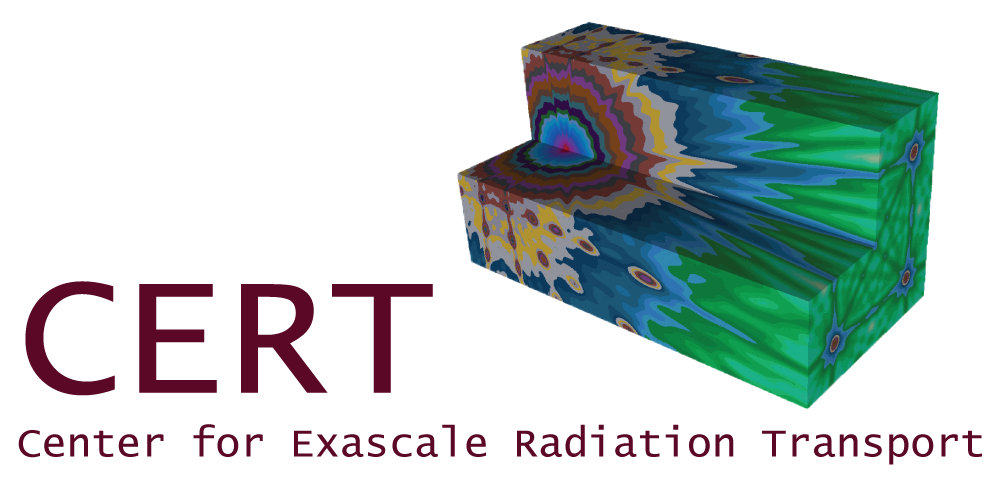
\includegraphics[height=0.18\textheight]{cert_logo_maroon.png}\end{tabular}}
%Michigan-themed
%\pgfdeclareimage[height=0.1in]{UMlogo}{michigan_engineering.png}
%\logo{\raisebox{-8pt}{\pgfuseimage{UMlogo}}}
%\titlegraphic{
\includegraphics[height=0.2\textheight]{michigan_block_m.png}}


%%%%%%%%%%%%%%%%%%%%%%%%%%%%%%%%%%%%%%%%%%%%%%%%%%%%%%%%%%%%%%%
% Optional packages, used to show off certain tricks

\newlength \figwidth
\setlength \figwidth {0.5\textwidth}


%%%%%%%%%%%%%%%%%%%%%%%%%%%%%%%%%%%%%%%%%%%%%%%%%%%%%%%%%%%%%%%

\usepackage[english]{babel}
\usetheme{boxes}

%Make it Aggie Maroon
\usecolortheme[RGB={80,0,0}]{structure}  
%Or Michigan Blue
%\usecolortheme[RGB={0,0,153}]{structure}  
%Or Michigan Maize
%\usecolortheme[RGB={255,204,0}]{structure}  


\setbeamertemplate{headline}{}
\setbeamertemplate{navigation symbols}{}%remove navigation symbols
\setbeamertemplate{footline}[frame number]



\setbeamersize{text margin left=1cm}
\setbeamersize{text margin right=0.75 cm}

\makeatletter
\let\old@rule\@rule
\def\@rule[#1]#2#3{\textcolor{rulecolor}{\old@rule[#1]{#2}{#3}}}
\makeatother

\definecolor{rulecolor}{RGB}{80,0,0}


  % This will typeset only the frames (or slides) that have the given label ("current" in this case).

\title[HOLO for TRT]{A High-Order Low-Order Algorithm with Exponentially-Convergent Monte Carlo for
    Thermal Radiative Transfer}
    \author[S.R. Bolding]{{Simon Bolding, Matt Cleveland, and Jim Morel}}
\date{{4 August 2016} }
\subject{}
%\institute{Los Alamos National Laboratory}

% \classificationlevel{SECRET/RD}
% \transmissible{}

%\reportnum{\textcolor{blue}{SAMPLE TEMPLATE ONLY \\ Contains NO Classified
%Information}}

% \dissableframenumber
\begin{document}
\setbeamercolor*{title}{use=structure,fg=white,bg=structure.fg}
\setbeamertemplate{title page}[default][colsep=-4bp,rounded=true,shadow=true]

\def\beginpage{\null\vfill\bgroup
\offinterlineskip\leftskip=\z@}
\def\endpage{\egroup\eject}

\begin{frame}
    \titlepage \vspace{-0.213in}
    \begin{center}
    \end{center}    
\end{frame}

\setlength{\tabcolsep}{6pt}

\setbeamercolor*{frametitle}{fg=Black!78}


%%%%%%%%%%%%%%%%%%%%%%%%%%%%%%%%%%%%%%%%%%%%%%%%%%%%%%%%%%%%%%%%%%%%%%%%%%%%%%%%%%%%%%%%%
\begin{frame}
\frametitle{We are interested in modeling thermal radiation transport \\ in the high energy
    density physics regime}
{\addtolength{\leftmargini}{-0.2in}
    \addtolength{\wideitemsep}{0.08in}
\begin{itemize}
    \item[] Modeling materials under extreme conditions \\ \colG{Temperatures $\mathcal{O}(10^6)$ K or more}
    \item[] Photon radiation transports through a material \\ 
        \colG{Significant \colb{energy}  may be exchanged}
 \item[] We want to improve efficiency of Monte Carlo calculations \\
     \colG{e.g., inertial confinement fusion, supernovae, et. al.}
    \end{itemize}}
\end{frame}


%%%%%%%%%%%%%%%%%%%%%%%%%%%%%%%%%%%%%%%%%%%%%%%%%%%%%%%%%%%%%%%%%%%%%%%%%%%%%%%%%%%%%%%%%
{\addtolength{\leftmargini}{-0.2in}
\begin{frame}
\frametitle{Our method has been applied to a simplified model:\\ the 1D
    frequency-integrated radiative
transfer equations}
\setlength{\unitlength}{\textwidth}
\vspace{0.152in}
\begin{itemize}
    \item[] Energy balance equations for radiation and material. \\
            \colG{Radiation intensity $I(x,\mu,t)$, material 
            temperature $T(x,t)$}\vspace{-0.34in}
    \item[] \begin{align*}\label{ho_cont}
\hspace{-0.134in}
    \frac{1}{c}\pderiv{I}{t} + \mu \pderiv{I}{x} + \sigma_t I(x,\mu,t)
    &= \frac{1}{4\pi} \sigma_a a c T^4,
  \\
  C_v \pderiv{T(x,t)}{t} &=  \highlight{\sigma_a \phi(x,t)} - \highlight{\sigma_a a c T^4}\\
\end{align*}
            \vspace{-0.34043in}
        \item[] Equations are \colb{nonlinear} and may be tightly coupled \\  
            \colG{Absorption opacity ($\sigma_a$) can be a strong function of $T$}
%        \item[] For practical applications, spatial discretizations \\ must preserve the \colb{equilibrium diffusion limit} (EDL)
\end{itemize}
\end{frame}
}

%%%%%%%%%%%%%%%%%%%%%%%%%%%%%%%%%%%%%%%%%%%%%%%%%%%%%%%%%%%%%%%%%%%%%%%%%%%%%%%%%%%%%%%%%
\begin{frame}
    \frametitle{Implicit Monte Carlo (IMC) is the standard Monte Carlo transport method for TRT problems}
        \vspace{-0.2in}
\begin{itemize}
    \item[] The system is \emph{linearized} over a time step $t\in[t^n,t^{n+1}]$ \\ 
        \colG{Opacities are evaluated with $T(t^n)$}\vspace{0.21in}
\setlength\wideitemsep{0.2in}
    \begin{itemize}
        \item Produces a linear transport equation
               \\ \colG{with effective emission and scattering terms}
        \item MC particle histories are simulated 
            \\ \colG{tallying radiation energy deposition}
        \item Emission source is \textbf{not} fully time-implicit.\\
            \colG{Uses MC integration over $\Delta t$ for intensity}
    \end{itemize}
\end{itemize}
\end{frame}

\begin{frame}
\frametitle{We developed a \colb{high-order low-order (HOLO) method} \\ that improves on several drawbacks of IMC}
    \begin{center}
{\footnotesize
\begin{tabular}{p{0.5\textwidth} p{0.5\textwidth}} 
    \multicolumn{1}{l}{\textbf{\normalsize Standard  IMC}} & \multicolumn{1}{l}{\textbf{\normalsize
    HOLO Method}} \\ \hline [2pt]
    \parbox{0.4\textwidth}{Large \colr{statistical noise} possible} & 
    \parbox{0.5\textwidth}{ECMC is \colb{very statistically efficient} \\for TRT problems} \\ [\tabsep]
 \parbox{0.4\textwidth}{{\color{red}Effective scattering} can make \\ MC  very expensive}
 & \parbox{0.4\textwidth}{MC solution has \colb{no
 scattering}} \\[\tabsep] 
 \parbox{0.5\textwidth}{Linearization can cause \colr{non-physical}\\ results  (maximum principle
 violations)} & \parbox{0.5\textwidth}{Fully \colb{implicit} time-discretization
 and \\ LO solution \colb{resolves nonlinearities}} \\[\tabsep] 
 \parbox{0.5\textwidth}{\colG{Reconstruction of linear emission shape limits artificial energy propagation}} &
 \parbox{0.5\textwidth}{Linear-discontinuous FE for $T(x)$ \\ preserving equilibrium diffusion limit} 
\end{tabular}
}
\end{center}
\end{frame}

\begin{frame}<*>
    \frametitle{\shorttitle}
        \vspace{0pt}
        \begin{minipage}[c][0.6\textheight]{0.2\textwidth}
            \hspace{-2em}
\includegraphics[width=\textwidth]{tamu_seal.png}\hspace{1em}
            \rule[-0.3\textheight]{1pt}{0.8\textheight}
        \end{minipage}
    \vspace{0pt}
        \begin{minipage}[c][0.6\textheight]{0.74\textwidth}
\tableofcontents[
hideothersubsections,
sectionstyle=show,
subsectionstyle=hide
]
         \end{minipage}
\end{frame}
%%%%%%%%%%%%%%%%%%%%%%%%%%%%%%%%%%%%%%%%%%%%%%%%%%%%%%%%%%%%%%%%%%%%%%%%%%%%%%%%%%%%%%%%%
\section{Overview of algorithm}

%%%%%%%%%%%%%%%%%%%%%%%%%%%%%%%%%%%%%%%%%%%%%%%%%%%%%%%%%%%%%%%%%%%%%%%%%%%%%%%%%%%%%%%%%
\begin{frame}
    \frametitle{Basic idea is a nonlinear low-order system with high-order angular correction from Monte Carlo transport solves}
    \setlength{\unitlength}{1mm}
    \begin{picture}(120,80)(0,-84)
    \put(-5,-15){
    \begin{minipage}[t]{1.1\textwidth}
        \begin{itemize}
\setlength\wideitemsep{0.2in}
            \item[] The \textbf{LO system} is space-angle moment equations,\\
                    \colG{on a fixed finite-element (FE) spatial mesh}
                \vspace{0.02in}
                {\scriptsize
                \begin{itemize}
                    \item Reduced dimensionality in angle\\
                         \colG{allows for solution with Newton's method}
                     \item \textbf{Output:} linear-discontinuous  $\phi(x)$ and $T(x)$\\ 
                         \colb{Construct LDFE scattering and emission source}
                  %  \item Consistency terms derived directly from transport equation
                \end{itemize}
}\vspace{0.2in}
            \item[] The \textbf{HO system} is a pure-absorber transport problem
                {\scriptsize
                \begin{itemize}
                    \item Solved with exponentially-convergent MC (ECMC) \\ \colG{for
                            \emph{efficient} reduction of statistical noise }
                    \item \textbf{Output:} \colb{consistency terms} \\
                \end{itemize}
}
        \end{itemize}
    \end{minipage}

}
\end{picture}
\end{frame}


\begin{frame}
    \frametitle{Iterations between the HO and LO systems \\ can be performed each time step}
    %\fontsize{9}{5.0}\selectfont
        \hspace{-0.1in}
        \resizebox{1.04\linewidth}{!}{
    \fontsize{10}{12.0}\selectfont
    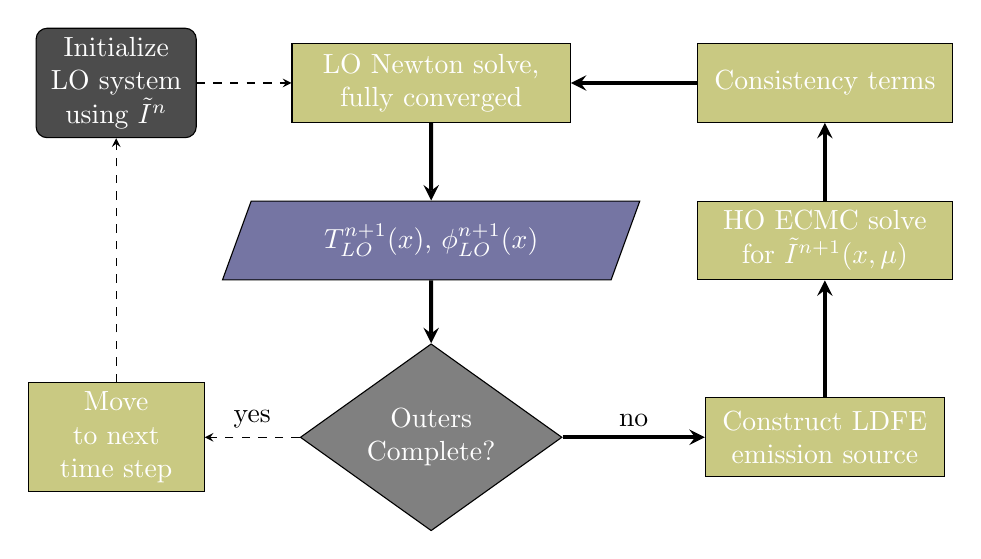
\begin{tikzpicture}[node distance=2cm]
        \node (start) [startstop] {Initialize LO system using $\tilde{I}^n$};
        \node (in1) [process, right of=start, xshift=2cm, text width=3.3cm]  {
        {LO Newton solve, fully converged}};
        \node (pro1) [io, below of=in1] {$T_{LO}^{n+1}(x)$, $\phi_{LO}^{n+1}(x)$};
        \node (dec1) [decision, below of=pro1, yshift=-0.5cm, text width=1.74cm] {Outers Complete?};
        \node (pro2a) [process, left of=dec1, xshift=-2.0cm] {Move to next time
        step};
        \node (srcs) [process, right of=dec1, xshift=3.0cm, text width=2.8cm] {
        {Construct LDFE emission source}};
        \node (pro2b) [process, text width=3.0cm, above of=srcs, yshift=0.5cm] {{HO ECMC solve}
           for $\tilde I^{n+1}(x,\mu)$};
        \node (cons) [process, above of=pro2b, text width=3.0cm] {{Consistency
        terms}};
        \draw [arrow1] (start) -- (in1);
        \draw [arrow] (in1) -- (pro1);
        \draw [arrow] (pro1) -- (dec1);
        \draw [arrow] (srcs) -- (pro2b);
        \draw [arrow] (dec1.east) -- node[anchor=south] {no} (srcs);
        \draw [arrow1] (dec1.west) -- node[anchor=south] {yes} (pro2a);
        \draw [arrow1] (pro2a) -- (start);
        \draw [arrow] (pro2b) -- (cons);
        \draw [arrow] (cons) -- (in1);
    \end{tikzpicture}
}
\end{frame}


%%%%%%%%%%%%%%%%%%%%%%%%%%%%%%%%%%%%%%%%%%%%%%%%%%%%%%%%%%%%%%%%%%%%%%%%%%%%%%%%%%%%%%%%%
%\begin{frame}
%    \frametitle{High-Order Low-Order Algorithm}
%    %\fontsize{9}{5.0}\selectfont
%        \resizebox{0.99\linewidth}{!}{
%    \fontsize{10}{12.0}\selectfont
%    \begin{tikzpicture}[node distance=2cm]
%        \node (start) [startstop] {Initialize LO system using ${I}^n$};
%        \node (in1) [process, right of=start, xshift=2cm, text width=3.3cm]  {
%        {LO Newton solve, fully converged}};%{LO solve:\vspace{0.041in}        $\B D(\mu^{HO})\Phi = \frac{1}{\keff}\B F\Phi$};
%        \node (pro1) [io, below of=in1] {$T_{LO}^{n+1}(x)$, $\phi_{LO}^{n+1}(x)$};
%        \node (dec1) [decision, below of=pro1, yshift=-0.5cm, text width=1.74cm] {Outers Complete?};
%        \node (pro2a) [process, left of=dec1, xshift=-2.0cm] {Move to next time
%         step};
%        \node (srcs) [process, right of=dec1, xshift=3.0cm, text width=2.8cm] {
%        {Construct LD sources}};
%        \node (pro2b) [process, above of=srcs, yshift=0.5cm] {{HO ECMC Solve}};
%        \node (cons) [process, above of=pro2b, text width=3.0cm] {{Compute consistency
%        terms}};
%        \draw [arrow1] (start) -- (in1);
%        \draw [arrow] (in1) -- (pro1);
%        \draw [arrow] (pro1) -- (dec1);
%        \draw [arrow] (srcs) -- (pro2b);
%        \draw [arrow] (dec1.east) -- node[anchor=south] {no} (srcs);
%        \draw [arrow1] (dec1.west) -- node[anchor=south] {yes} (pro2a);
%        \draw [arrow1] (pro2a) -- (start);
%        \draw [arrow] (pro2b) -- (cons);
%        \draw [arrow] (cons) -- (in1);
%    \end{tikzpicture}
%}
%\end{frame}





\section{Derivation of the LO equations}
\subsection{}


%%%%%%%%%%%%%%%%%%%%%%%%%%%%%%%%%%%%%%%%%%%%%%%%%%%%%%%%%%%%%%%%%%%%%%%%%%%%%%%%%%%%%%%%%
\begin{frame}
    \frametitle{The LO equations are formed as \emph{consistently} as possible with spatial and
    angular moments of TRT equations}
    \begin{itemize} \vspace{0.15in}
        \item[] The time discretization is backward Euler\\ \colG{for both the HO and LO equations}
        \item[] Spatial moments are weighted with FE basis functions:   \end{itemize}
    \begin{columns}
        \begin{column}{0.5\textwidth}
    \begin{centering}
        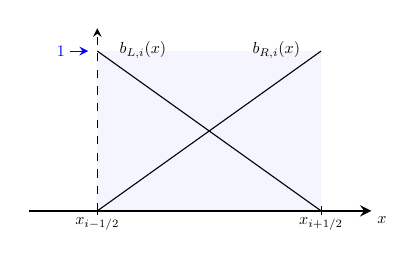
\begin{tikzpicture}[scale=0.58, every node/.style={transform shape}]
            \fill[fill=blue!20!white!20] (11.0,0.5) rectangle (15.90,4.0);
            \node at (10.4,4.0) {$\colb{1}$ \hspace{0.8em} };
            \draw [Blue,->] (10.4,4.0) -- (10.8,4.0);
            \draw (11.0,0.4) -- (11.0,0.6) node[below, pos=0.4] {$x_{i-1/2}$};
            \draw (15.90,0.4) -- (15.90,0.6) node[below, pos=0.4] {$x_{i+1/2}$};
            \node at (14.92,4.02) {$b_{R,i}(x)$};
            \node at (12.0,4.02) {$b_{L,i}(x)$};
            \draw [thick,->] (9.5,0.5) -- (17.0,0.5) node[anchor=north west] {$x$};
            \draw [dashed,->] (11.0,0.5) -- (11.0,4.5);
            \draw (11.0,0.5) -- (15.90,4.0);
            \draw (15.90,0.5) -- (11.0,4.0);
        \end{tikzpicture}
    \end{centering}
        \end{column}
        \begin{column}{0.5\textwidth}
        \begin{equation*}
        \boxed{\displaystyle \mom{\cdot}_{L,i} = \frac{2}{h_i} \int_{x_\il}^{x_\ir}
        b_{L,i}(x)(\cdot) \d x \quad }  
        \end{equation*}
    \end{column}
\end{columns}
\begin{itemize}
        \vspace{0.2in}
    \item[] Half-range integrals reduce angular dimensionality
    \begin{equation*}
        \boxed{{\displaystyle I^+(x) =
        2\pi\int_0^1 I(x,\mu) \d \mu}}
    \end{equation*}
\end{itemize}
\end{frame}


%%%%%%%%%%%%%%%%%%%%%%%%%%%%%%%%%%%%%%%%%%%%%%%%%%%%%%%%%%%%%%%%%%%%%%%%%%%%%%%%%%%%%%%%%
\begin{frame}
    \frametitle{Apply moments to the TRT equations \\ and manipulate to form
        \colb{angular consistency
    terms}}
    {\addtolength{\leftmargini}{-1.2cm}
    \begin{itemize}
%        \item[] Ultimately, we get 4 radiation and 2 material equations \\
%            \colG{for each spatial element $i$}
%        \item[] The streaming terms are algebraically manipulated \\ 
%            \colG{to form consistency terms (\colb{no approximation here})}
%            \vspace{0.3cm}
%            \pause
        \item[]  {For example, apply $\mom{\cdot}_{L,i}^+$ to a streaming term:}
    \end{itemize}$
    \fontsize{9.2}{13.0}\selectfont
    \begin{array}{lll}
        {\displaystyle \left \langle \mu \pderiv{I}{x} \right \rangle_L^+ } & = & -\frac{\ds2}{\ds h_i} \{ \mu I \}_{i-1/2}^+ +
        \frac{\ds 1}{\ds h_i}\left[\mom{\mu I}_{L,i}^+ + \mom{\mu I}_{R,i}^+\right] \\
        & = & -\frac{\ds2}{\ds h_i} \highlight{\frac{\ds\{ \mu I
        \}^+_{i-1/2} }{\ds I^+_{i-1/2}}}
        I^+_{i-1/2} + \frac{\ds 1}{\ds h_i} \highlight{\frac{\ds\mom{\mu
        I}_{L,i}^+}{\ds\mom{I}_{L,i}^+}}\mom{I}_{L,i}^+  +
        \frac{\ds 1}{\ds h_i}\highlight{\frac{\ds\mom{\mu
        I}_{R,i}^+}{\ds\mom{I}_{R,i}^+}}\mom{I}_{R,i}^+  
            \end{array}$
    \pause
    \begin{itemize}
            \vspace{0.3in}
        \item[] Now, close the final moment equations:
        \begin{itemize}
                \vspace{0.1in}
        \item Approximate consistency terms with \colb{ $\tilde{I}_{\text{HO}}^{n+1}$} \\
            \colG{from previous HO solve}
                \vspace{-0.1in}
    \item Eliminate remaining face unknowns with LD spatial closure
        \colG{$T^4(x)$ and $T(x)$ also assumed LD}
    \end{itemize}
    \end{itemize}
}
\end{frame}




\section{Exponentially Convergent MC High-Order Solver}
\subsection{}

%%%%%%%%%%%%%%%%%%%%%%%%%%%%%%%%%%%%%%%%%%%%%%%%%%%%%%%%%%%%%%%%%%%%%%%%%%%%%%%%%%%%%%%%%%
%{\addtolength\leftmargini{-0.165in}
%\begin{frame}
%    \frametitle{Exponentially Convergent Monte Carlo \\ can efficiently reduce noise globally}
%    \begin{itemize}
%            \addtolength{\wideitemsep}{0.14in}
%        \item[] Each MC batch tallies the \colb{error} in the solution 
%            \begin{itemize}
%                \item \colG{standard MC particle transport,\\ but a \colr{complex} source}
%                    \vspace{-0.21in}
%                \item \colG{ECMC requires  a \colr{functional} representation of $I(x,\mu)$}
%    \end{itemize}
%
%        \item[] Can reduce solution error \colb{globally} $\propto e^{-\alpha N}$ \\
%            \colG{Adaptive $h$-refinement can help represent error}
%        \item[] $I^{n}(x,\mu)$ often provides an \colb{\textbf{excellent}} estimate of
%            $I^{n+1}(x,\mu)$\\  \colG{No MC sampling from thermal equilibrium regions}
%     \end{itemize}
% \end{frame}
% }



%%%%%%%%%%%%%%%%%%%%%%%%%%%%%%%%%%%%%%%%%%%%%%%%%%%%%%%%%%%%%%%%%%%%%%%%%%%%%%%%%%%%%%%%%
 \begin{frame}
 \frametitle{We use a \colb{projection} $\tilde I(x,\mu)$ onto a \\ space-angle LDFE  mesh to represent the solution}
     \begin{itemize}
         \item[] 
{\small
    \begin{minipage}[c]{0.9\linewidth}
        \vspace{33pt}
             \begin{equation*}
                 \tilde{I}_{ij}(x,\mu) = \  \tikzmark{moma}{\colb{I_{a}}}\ + \frac{2}{h_x}\;\tikzmark{momx}{\colb{I_{x}}}\  (x-x_i) +
                 \frac{2}{h_\mu} \  \tikzmark{mommu}{\colb{I_{\mu}}}\  (\mu-\mu_i)
             \end{equation*}
        \begin{tikzpicture}[overlay, remember picture]
    \node (descr) at (4,1.8) {local volumetric tallies};
    \draw[,->,thick,Gray!60] (descr) to [in=90,out=-90] (moma);
    \draw[,->,thick,Gray!60] (descr) to [in=90,out=-90] (momx);
    \draw[,->,thick,Gray!60] (descr) to [in=90,out=-90] (mommu);
        \end{tikzpicture}
    \end{minipage}
}
    \end{itemize}
\vspace{0.1in}
   { \setlength\unitlength{1mm}
    \begin{picture}(130mm,40mm)
    \put(-4,40){
    \begin{minipage}[t]{0.6\linewidth}
        \vspace{0pt}
        \centering
        \scalebox{0.7}{
        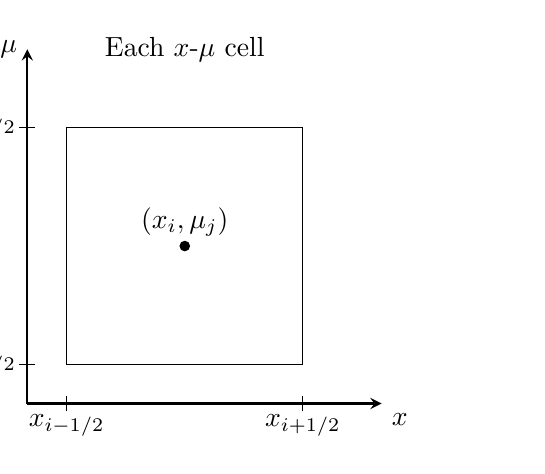
\begin{tikzpicture}
            \hspace{-0.5in}
            \draw (1,1) rectangle (4,4);
            \node[draw,circle,inner sep=1.2 pt,fill] at (2.5,2.5) {};
            \node[above] at (2.5,2.5) {$(x_i,\mu_j)$};
            \node at (2.5,5.0) {Each $x$-$\mu$ cell};
            \draw (1.0,0.4) -- (1.0,0.6) node[below, pos=0.4] {$x_{i-1/2}$};
            \draw (4.0,0.4) -- (4.0,0.6) node[below, pos=0.4] {$x_{i+1/2}$};
            \draw (0.4,1.0) -- (0.6,1.0) node[left, pos=0.4] {$\mu_{j-1/2}$};
            \draw (0.4,4.0) -- (0.6,4.0) node[left, pos=0.4] {$\mu_{j+1/2}$};
            \draw [thick,->] (0.5,0.5) -- (5,0.5) node[anchor=north west] {$x$};
            \draw [thick,->] (0.5,0.5) -- (0.5,5) node[anchor=east] {$\mu$};
        \end{tikzpicture}
    }
    \end{minipage}} 
    \put(55,0){\centering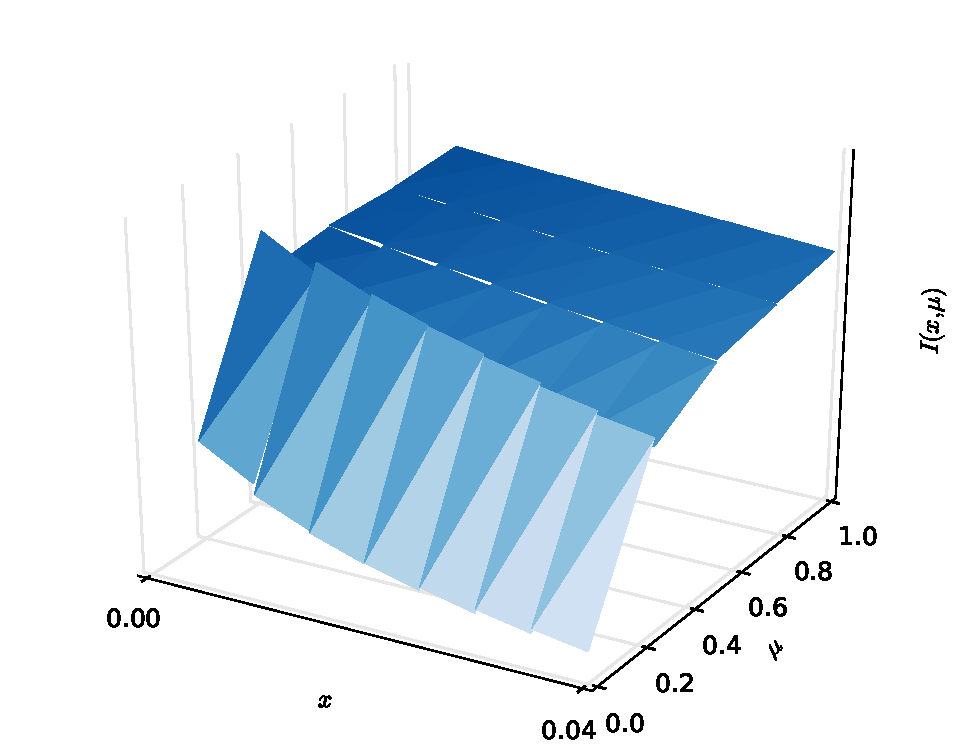
\includegraphics[trim=0.0in 0.0in 0.0in 0.5in,clip,width=0.55\textwidth]{zoom_angflux.pdf}
        }
    \end{picture}}
\end{frame}


%%%%%%%%%%%%%%%%%%%%%%%%%%%%%%%%%%%%%%%%%%%%%%%%%%%%%%%%%%%%%%%%%%%%%%%%%%%%%%%%%%%%%%%%%
\begin{frame}
    \frametitle{We apply the ECMC algorithm to \\ the \colb{pure-absorber} HO transport equation}
        \vspace{-0.05in}
        \begin{align*}
            \hspace{-0.2in}
            \left[\mu \pderiv{}{x} + \left(\sigma_t+\frac{1}{c\Delta t}\right)\right]I^{n+1}
            &=  \frac{1}{4\pi}\left[\highlight{\sigma_a a c
    \left(T_{LO}^{n+1}\right)^4+\sigma_s\phi_{LO}^{n+1}}\right]+ \frac{\tilde I^{n}}{c\Delta t}  \\[5pt]
            \B L I^{n+1} &= q
     \end{align*}
        \begin{block}{For each batch $m$:}
         \begin{itemize}
        \item Evaluate residual source: $r^{(m)} = q - \B L \tilde I^{n+1,(m)}$
        \item Estimate ${\epsilon}^{(m)} = \B L^{-1} {r}^{(m)}\;\;$ via \colb{MC simulation}    
 %       \item Update solution:\vspace{-0.08in} \begin{align*}\tilde I^{n+1,(m+1)} &= \tilde I^{n+1,(m)} + \tilde \epsilon^{(m)} \\ 
 %                                                 &= \colG{\tilde I^{n+1,(m)} + \B L^{-1} q - \B L^{-1} \B L \tilde
 %   I^{n+1,(m)}}\end{align*}
        \item Update solution: $\tilde I^{n+1,(m+1)} = \tilde I^{n+1,(m)} + \tilde \epsilon^{(m)}$
    \end{itemize}
\end{block}
\end{frame}


%%%%%%%%%%%%%%%%%%%%%%%%%%%%%%%%%%%%%%%%%%%%%%%%%%%%%%%%%%%%%%%%%%%%%%%%%%%%%%%%%%%%%%%%%
\begin{frame}
    \frametitle{I implemented straight-forward variance reduction \\ straight-forward variance reduction}
    \addtolength{\wideitemsep}{0.15in}
    \begin{itemize}
        \item[] $I^{n}(x,\mu)$ is often an \colb{\textbf{excellent}} estimate of
            $I^{n+1}(x,\mu)$\\  \colG{No MC sampling from thermal equilibrium regions}
        \item[] Histories stream without collision \\
            \colG{along path $s$, weight reduces as $w(s)=w_0 e^{-\sigma_t s}$}
        \item[] Use cell-wise {systematic} sampling for $|r^{(m)}|$ source
            \colG{Particularly effective in thick cells}
            \begin{itemize}
                    \vspace{0.02in}
                \item Particles in  each $x$-$\mu$ cell $\propto |r^{(m)}|$ in cell
                \vspace{-0.15in}
                \item Set minimum $n$ for cells  \\
                    \colG{except for cells in thermal equilibrium}
            \end{itemize}
    \end{itemize}
\end{frame}


\section{Computational Results}
\subsection{}




\begin{frame}
    \frametitle{We will test our method with several \\ standard \textbf{Marshak Wave} problems}
    {\setlength\unitlength{1mm}
    \begin{picture}(150mm,80mm)(0,0)
    \put(0,20){
    \begin{minipage}[t]{\linewidth}
        \vspace{0pt}
        \begin{itemize}
            \item[] Figures depict \colb{radiation temperature} $T_r = \sqrt[4]{\phi/ac}$
        \end{itemize}
    \end{minipage}} 
    \put(0,30){\centering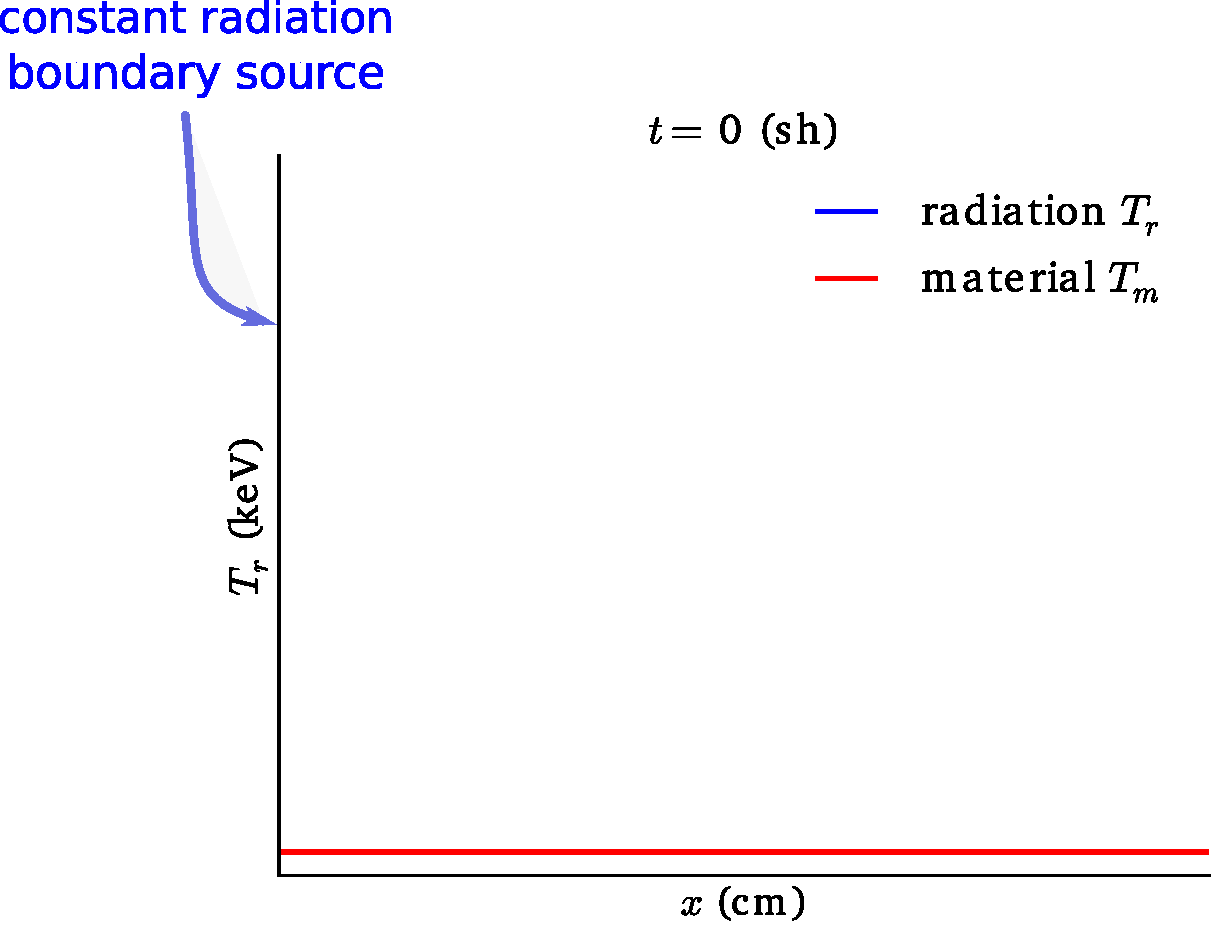
\includegraphics[trim=0.0in 0.0in 0.0in
    0.0in,clip,width=0.485\textwidth]{start_time_labeled.pdf}}
    \put(65,30){\centering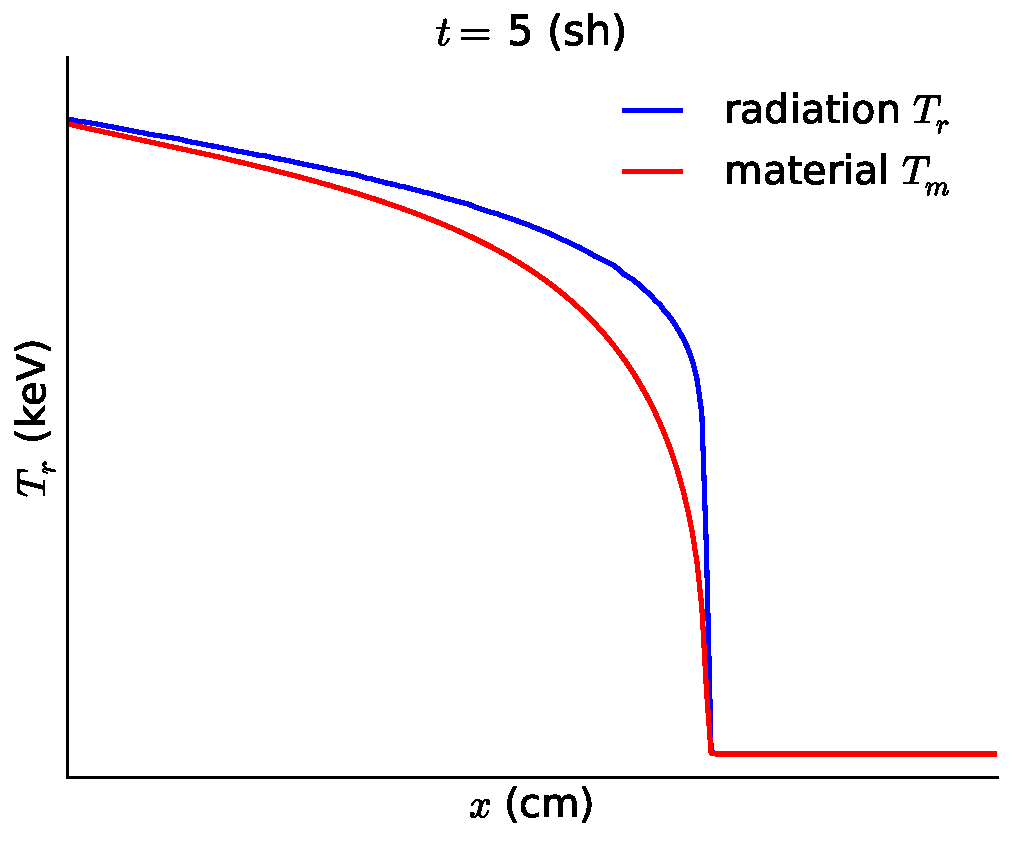
\includegraphics[trim=0.0in 0.0in 0.0in
    0.0in,clip,width=0.4\textwidth]{end_time.pdf}}
    \put(50,50){\tikz{\draw[->,line width=2mm,Gray!90] (0,0) -- (12mm,0);}}
\end{picture}}
\end{frame}

\begin{frame}
    \frametitle{Implementation specifics for results are given below:}               
    {\addtolength\wideitemsep{11pt}
    \begin{itemize}
    \item HOLO method implemented as stand-alone C++ code \\
        \colG{IMC results from Jayenne (LANL code)}
    \item $\Delta t$ increases from $0.01$ ns to $0.1$ ns
    \item One HO solve per time step, with two LO solves
        \begin{itemize}
            \item \emph{each HO} solve has 3 ECMC batches \\ \colG{no adaptive mesh refinement}
        \end{itemize}
    \item Figure of Merit: \boxed{\text{FOM}=\frac{\displaystyle 1}{\displaystyle
            \|\sigma_{\text{rel}}\|^2 N_{\text{total}}}}\\ \colG{are normalized to IMC results}
    \end{itemize}
    }
\end{frame}


%%%%%%%%%%%%%%%%%%%%%%%%%%%%%%%%%%%%%%%%%%%%%%%%%%%%%%%%%%%%%%%%%%%%%%%%%%%%%%%%%%%%%%%%%
\begin{frame}
    \frametitle{The HOLO method produces significantly less noise \\ than IMC for a typical Marshak Wave: \textbf{FOM=145}}
    \centering
        \begin{itemize}
            \item \colb{$\sigma_a\propto T^{-3}$} 
            \item Transient solution after 5 shakes ($\sim 520$ steps) \\ \colG{200~$x$ cells (and 4~$\mu$
                cells for ECMC)}
        \end{itemize}
    \begin{figure}
    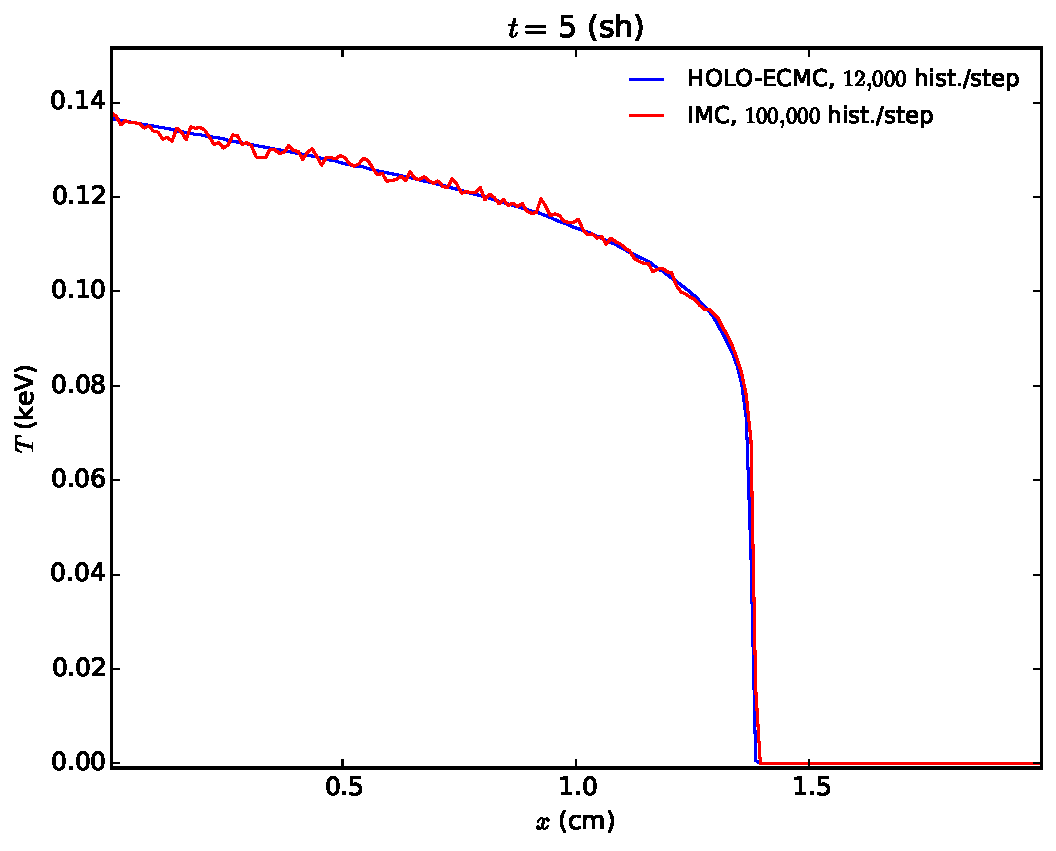
\includegraphics[width=0.615799\textwidth]{marshak_200_compare.pdf}
    \end{figure}
\end{frame}

%%%%%%%%%%%%%%%%%%%%%%%%%%%%%%%%%%%%%%%%%%%%%%%%%%%%%%%%%%%%%%%%%%%%%%%%%%%%%%%%%%%%%%%%%
%\begin{frame}
%    \frametitle{The LDFE representation has higher spatial accuracy \\ than IMC source tilting for two-material problem}
%        \fontsize{10.2pt}{10.2pt}\selectfont
%        \vspace{0.2in}
%        \begin{itemize}
%            \item[] Left half is optically thin ($\sigma\!=\!0.2$ cm$^{-1}$) and
%                right half is thick ($\sigma_a\!=\!2000$ cm$^{-1}$). \colG{ECMC uses 8 $\mu$ cells}
%        \end{itemize}
%\begin{figure}
%    \centering
%    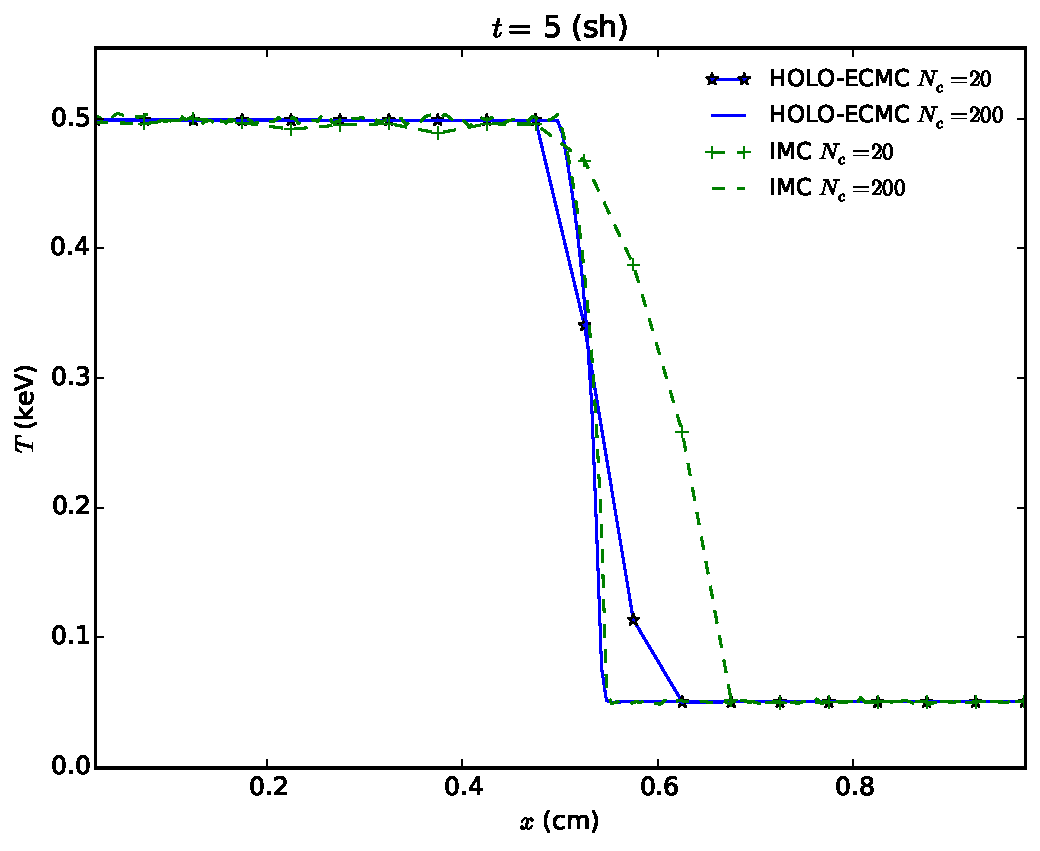
\includegraphics[width=0.6755799\textwidth]{two_mat_conv.pdf}
%\end{figure}
%
%\end{frame}

\begin{frame}
    \frametitle{ECMC is more efficient than\\
 standard MC  as a HO solver }
{\addtolength\leftmargini{-0.345in}
    \centering
        \fontsize{10.0pt}{10.2pt}\selectfont
        \vspace{0.2in}
        \begin{itemize}
            \item Left half is optically thin ($\sigma\!=\!0.2$ cm$^{-1}$),
                right half is thick ($\sigma_a\!=\!2000$ cm$^{-1}$). \colG{8 $\mu$ cells}
            \item Results for HOLO with different HO solvers:\\ \colb{ECMC} (FOM=10,000),  \colr{ standard MC}
            (FOM=0.46), and an \colg{ S$_2$}
            solution
        \end{itemize}
    \begin{figure}
        \vspace{-0.1in}
    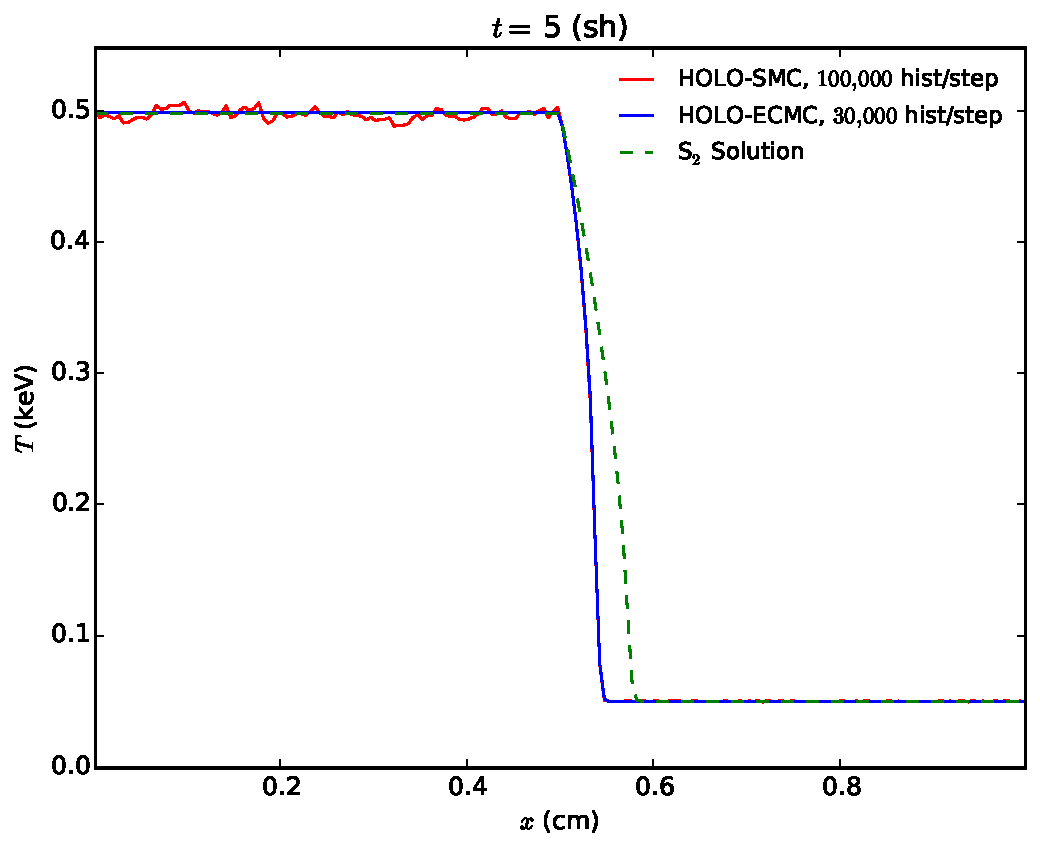
\includegraphics[width=0.6099\textwidth]{two_mat_ho_compare.pdf}
    \centering
    \end{figure}
}
\end{frame}

\begin{frame}
    \frametitle{The LDFE discretization for the LO equations \\ preserves the equilibrium diffusion limit}
        \begin{itemize}
            \item \colG{Large, constant $\sigma_a$ and small $c_v$}
        \end{itemize}
\begin{figure}
    \centering
    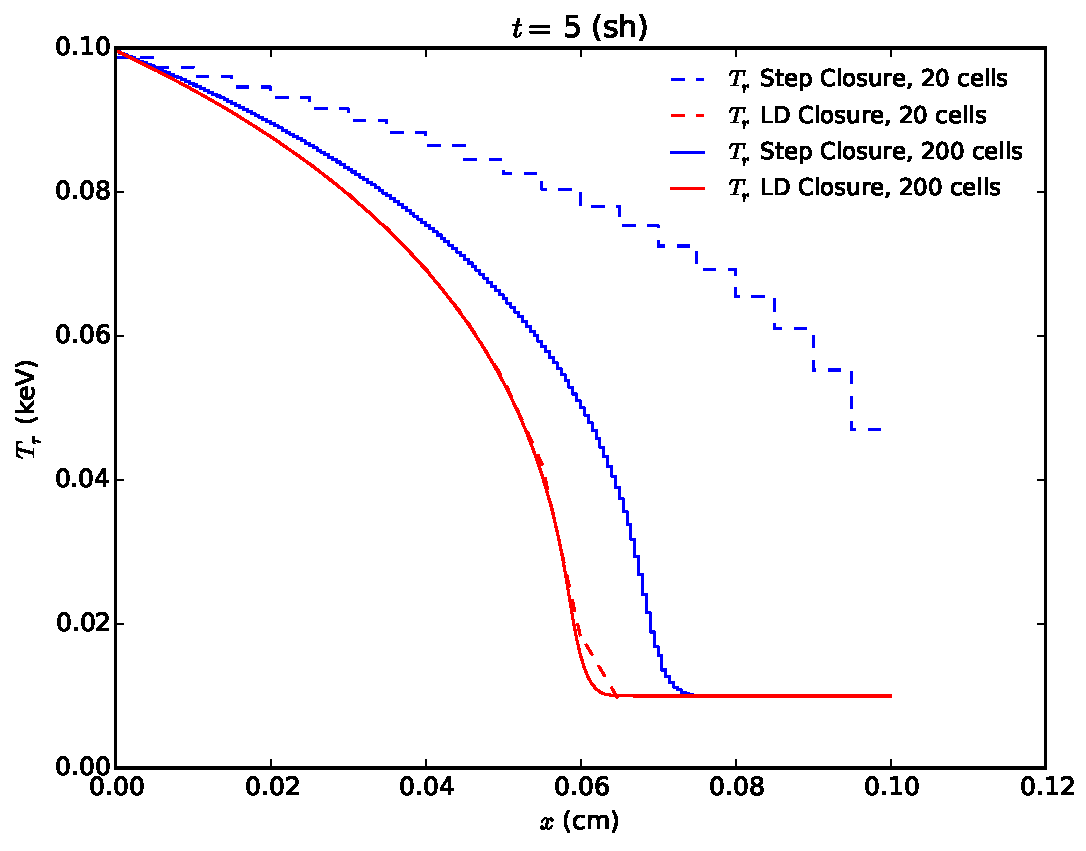
\includegraphics[width=0.6755799\textwidth]{diff_limit_compare.pdf}
\end{figure}
\end{frame}


\begin{frame}
    \frametitle{Our HOLO method preserves 
                the maximum principle\\ with sufficient nonlinear convergence}
                {
                    \vspace{0.01in}
    \addtolength{\leftmargini}{-1.2cm}
                    \begin{itemize}
    \fontsize{9.62}{12.0}\selectfont
    \vspace{0.1in}
\item \textbf{Material temperatures} plotted; all simulations end at $t=0.1$ sh \\
    \colG{$\sigma_a \propto T^{-3}$, $c_v$ small, $\Delta t \in [10^{-4},10^{-2}]$ sh}  
                        \vspace{-0.1in}
            \item LO Newton iterations required damping 
        \end{itemize}
            }
    \vspace{0.0in}
                
    \hspace{0.62in}
    {\setlength\unitlength{1mm}
    \begin{picture}(130mm,80mm)(0,0)
    \put(21,74){\underline{{IMC $T_m$}} }
    \put(00,30){\centering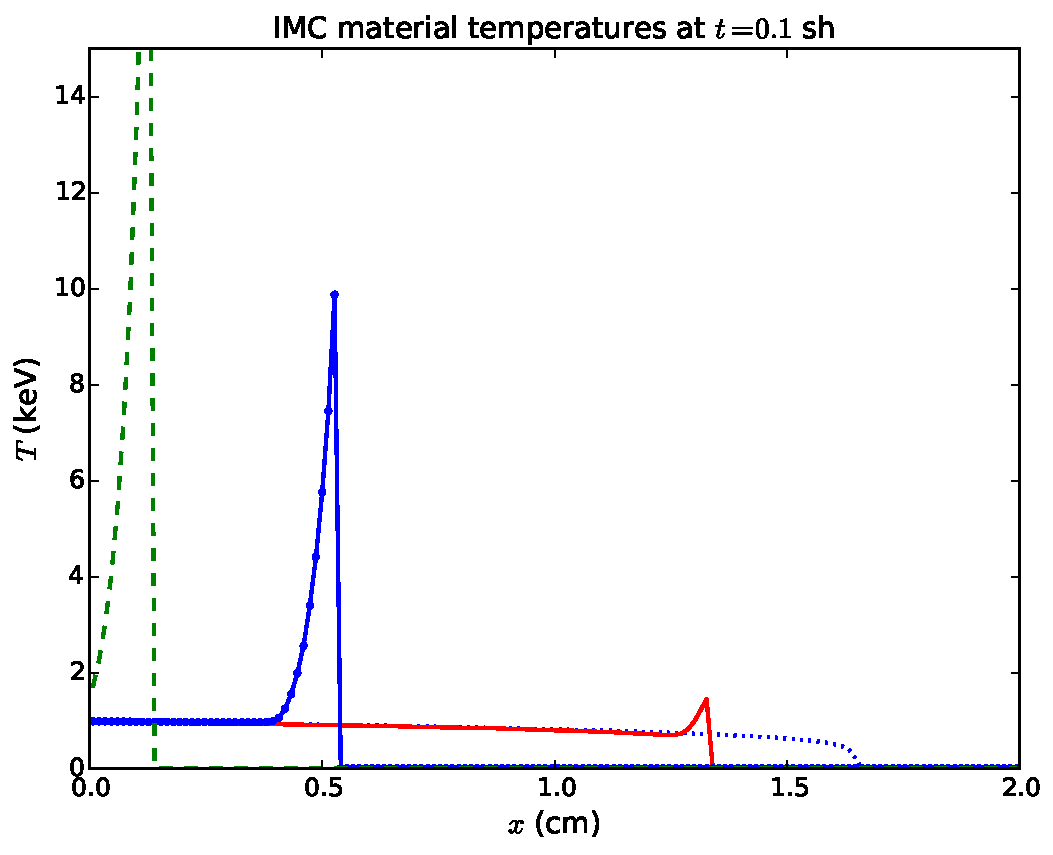
\includegraphics[trim=0.0in 0.0in 0.0in
    0.30in,clip,width=0.485\textwidth]{mpv_mats_imc_zoom.pdf}}
    \put(64.2,30){\centering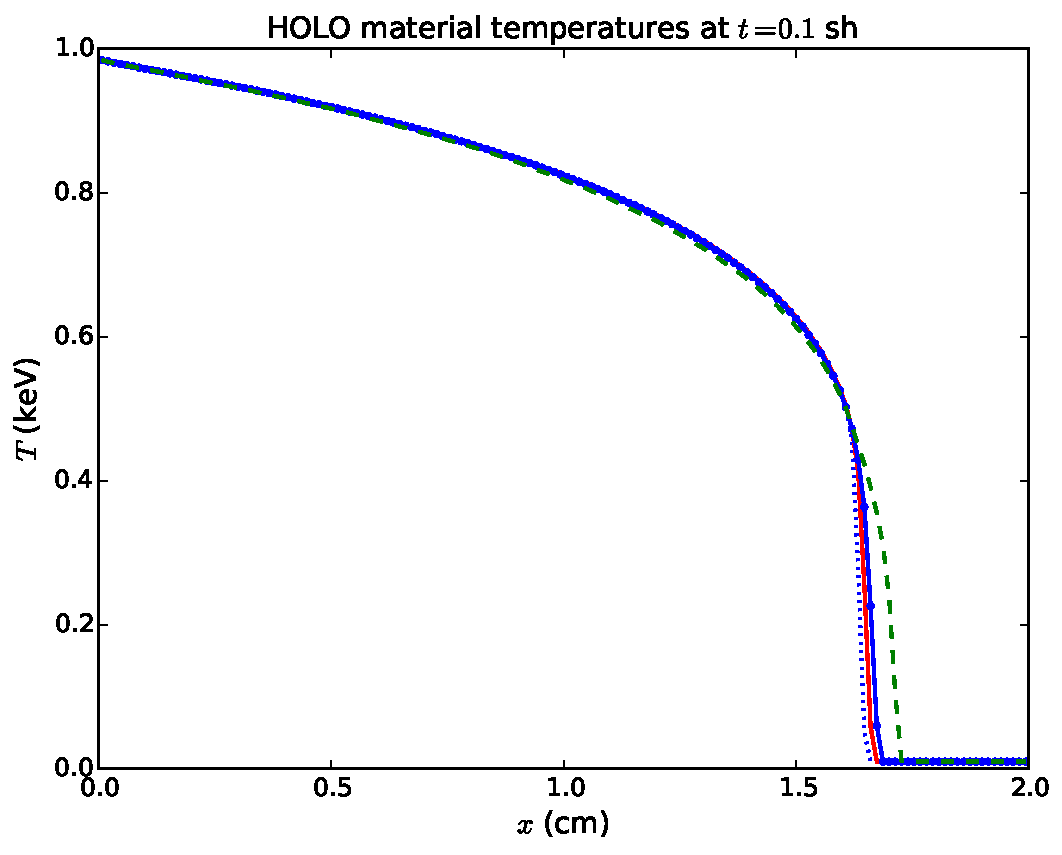
\includegraphics[trim=0.0in 0.0in 0.0in
    0.24in,clip,width=0.485\textwidth]{mpv_mats_holo_nolegend.pdf}}
    \put(85,74){\underline{{HOLO $T_m$}}}
    \put(30,40){\tikz{\draw[->,line width=0.3mm,black] (0,0) -- (-8mm,0);}}
    \put(28,42){\tiny $\Delta t$ increasing}
    \put(69,70.1){\tikz{\draw[fill=white,white] (0,0) rectangle (0.4\textwidth,2mm);}}
    \put(-7.8,36.0){\scriptsize {\color{Blue}$T_{r,\text{inc}}$}}
    \put(-0.7,36.5){\tikz{\draw[,->,line width=0.4mm,Blue] (20mm,0) -- (24mm,0);}}
    \put(56.5,69.3){\scriptsize {\color{Blue}$T_{r,\text{inc}}$}}
    \put(63.0,69.8){\tikz{\draw[,->,line width=0.4mm,Blue] (20mm,0) -- (23.5mm,0mm);}}
\end{picture}}

\end{frame}

\section{Extensions and Improvements on HOLO algorithm}

%\begin{frame}
%    \frametitle{We need a way to resolve issues when the LDFE representation of the intensity is
%        negative}
%    {\addtolength\wideitemsep{5pt}
%    \begin{itemize}
%        \item[] Negative intensities can occur in optically thick cells \\
%            \colG{Mesh refinement is of minimal use}
%        \item[] $\tilde I_{HO}(x,\mu)$ must be positive for consistency terms \\
%            \colG{to produce a physical, stable LO solution}
%         \item[] Independent fix up for LO solution
%             \colG{\\E.g., lumping or preserving balance with floored $\phi(x)$}
%    \end{itemize}
%}
%
%\end{frame}
%
%\begin{frame}
%    \frametitle{Can add source $\delta$ to produce a positive projection $\tilde I_{pos}$ 
%        such that $\tilde I_{pos}$ satisfies the
%    latest residual equation}
%    {\addtolength\wideitemsep{0.1in}
%    \begin{itemize} 
%        \item[] Produce $\tilde I_{\text{pos}}$ by scaling $x-\mu$ moments equally,
%            \\ \colG{to estimate source for the next iteration\vspace{0.1in}}
%            \begin{tikzpicture}
%                \hspace{-0.20771in}
%            \node at (0,0) {$\!\begin{aligned}
%                \B L \tilde I^{(m)}  &= q - r^{(m)} \\
%                    \B L \tilde I_{\text{pos}}^{(m)} &= q - r^{(m)} + \colb{\delta^{(m+1)}}
%            \end{aligned}$};
%             \node at (2.73,0.1) [fill=Gray!50,shape=single arrow,text width=0.7cm,text
%             height=0.00001cm,line width=0.01cm] {};
%             \node at (5.62,0){$\!\begin{aligned}
%                     \delta^{(m+1)} &= \B L \left(\tilde I^{(m)} - \tilde
%             I_{\text{pos}}^{(m)}\right)  \\
%             q &\rightarrow q + \delta^{(m+1)}
%            \end{aligned}$};
%            \end{tikzpicture}
%        \item[] We can delay error stagnation
%            \\ \colG{Investigating alternative positive projection of $I$}
%    \end{itemize}
%}
%\end{frame}


\begin{frame}
    \frametitle{The time variable can be included in the ECMC trial space \\ with a
    consistent LO time closure }
    \begin{columns}
        \begin{column}[t]{0.2\textwidth}
            \vspace{-20pt}
    \begin{center}
        \begin{tikzpicture}[scale=0.62, every node/.style={transform shape}]
            \node[anchor=south] at (1,4.0) {$\tilde{I}_{HO}^{n}$};
            \draw (1.0,4.0) node[fill,circle,inner sep=0pt,minimum
            size=4.2pt] {};
            \draw [->] (2.0,4.25) -- (3.0,4.25) node[anchor=west] {$t$};
            \draw (1.0,0.4) -- (1.0,0.6) node[below, pos=0.4] {$t^{n}$};
            \draw (5.90,0.4) -- (5.90,0.6) node[below, pos=0.4] {$t^{n+1}$};
            \node at (3.6,3.06) {$\overline{I}_{HO}(x,\mu)$};
            \draw [thick] (1.0,0.5) -- (5.9,0.5) node[anchor=north west] {};
            \filldraw[color=black, fill=white] (1,2.450) circle (2.1pt);
            \draw (1.0,2.45) -- (5.90,2.45);
            \filldraw[color=blue, fill=white] (5.9,2.450) circle (2.1pt);
            \draw (5.9,1.6) node[blue,fill,circle,inner sep=0pt,minimum size=4.2pt] {};
            \node[anchor=west] at (5.9,1.6) {${\color{blue}\tilde{I}_{HO}^{n+1}}$};
        \end{tikzpicture}
    \end{center}
    \end{column}
    \begin{column}[t]{0.85\textwidth}
    \vspace{0pt}
{\addtolength{\leftmargini}{-0.1in}
\fontsize{10.0pt}{9.0pt}\selectfont
    \begin{itemize}
        \item[] Include continuous $\frac{1}{c}\pderiv{}{t}\left(\cdot\right)$ in $\B L$ for residual
            source\\
            \colG{leaving $T(x)$ still implicit}
        \item[] Sample and track particle histories in time. \\ \colG{Tally the time-averaged and
                $t^{n+1}$ error}
        \vspace{0.08in}
    \item[] In \colb{LO equations}, parameterize $\phi_{LO}^{n+1}$ \\ in terms of
        \textbf{time-averaged}
        unknowns, e.g.,
            \begin{equation*}
                \mom{\phi}_{L,i}^{n+1} = 2\highlight{\gamma^{HO}_{L,i}} \overline{\mom{\phi}}_{L,i} -
                \mom{\phi}^{n}_{L,i}
            \end{equation*}
    \end{itemize}
}
    \end{column}      
    \end{columns}
\end{frame}

\begin{frame}
    \frametitle{The time-closure parameters preserve accuracy \\ of MC time integration  in the LO solution}
    \fontsize{10.0pt}{10.0pt}\selectfont
    \vspace{0.1in}
    \begin{itemize}
        \item Material is near-void, so temperature uncouples  \\ \colG{take 3 large time
                steps and compare $E_{R}^{n+1}=\phi^{n+1}/c$}
            \item 300,000 histories/step, 100 spatial cells
    \end{itemize}
    \begin{figure}
        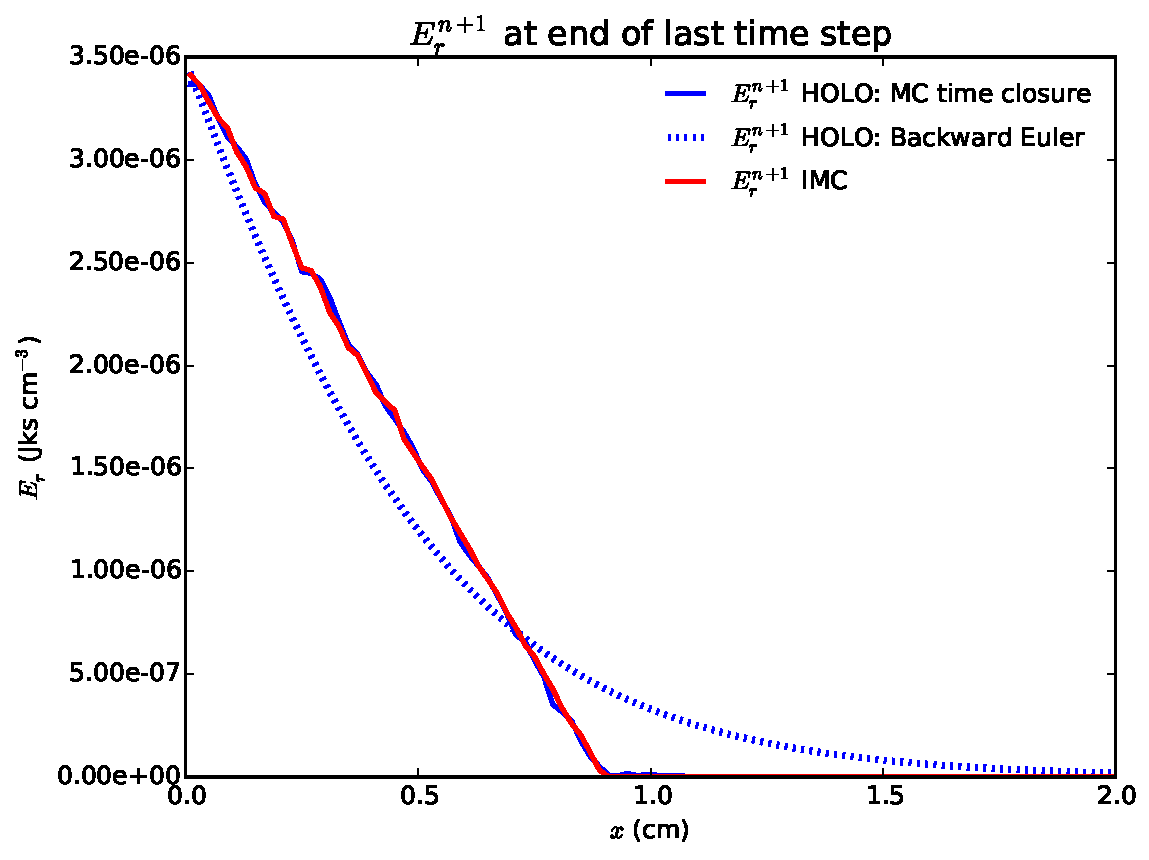
\includegraphics[width=0.71\textwidth]{void_compare_300k.pdf}
    \end{figure}
\end{frame}

\begin{frame}
    \frametitle{A few other potential improvements were investigated:}
    {\addtolength\wideitemsep{5pt}
        \begin{itemize}
            \item[] Resolving negative intensities in optically thick cells \\
            \colG{using an artificial source and alternate trial space}
        \item[] Using HO solution to estimate spatial closure \\
                \colG{by including face tallies in ECMC}
            \item[] Source iteration with diffusion synthetic acceleration \\ \colG{to
                    iteratively solve the LO equations}
        \end{itemize}}
\end{frame}


\begin{frame}
    \frametitle{\shorttitle}
    \begin{itemize}
        \item[] ECMC is very efficient for TRT simulations\\
            \colG{and fits well in global HOLO context}
        \item[] The LO system can resolve nonlinearities \\
            \colG{with bounded angular consistency terms}
        \item[] Next step is to extend to higher spatial dimensions \\
            \colG{main hurdle to overcome is infrastructure}
    \end{itemize} \pause
    \begin{tcolorbox}
    More details in: S.R. Bolding, M. Cleveland, and J.E. Morel. A HOLO Algorithm
with ECMC for Radiative Transfer. NS\&E: M\&C 2015 Special Issue, 2016. Accepted.
\end{tcolorbox}
\end{frame}


\titlegraphic{\centering\begin{tabular}{lr}\hspace{-2em}
\includegraphics[trim=0.0in 0.0in 0.0in 0.0in,clip,height=0.18\textheight]{NEUP.jpg} &
 \hspace{+2em}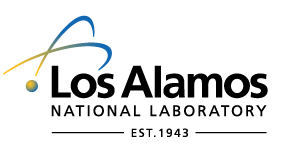
\includegraphics[trim=0.0in 0.4in 0.0in 0.0in,clip,height=0.18\textheight]{lanl-logo-footer.png} 
\end{tabular}}
\title{Simulations of Neutron Multiplicity Experiments with Perturbations to Nuclear Data}
    \author{Simon Bolding and C.J. Solomon}
\begin{frame}
    \maketitle
\end{frame}




\title{Simulations of Neutron Multiplicity Experiments with Nuclear Data Perturbations}
\author{S.R. Bolding\inst{1}, \and C.J. Solomon\inst{2}}
\institute[namemnae]{\inst{1} \textit{Texas A\&M University, College station, TX }
\and \vspace{-0.1in}\inst{2} \textit{Los Alamos National
Laboratory, Los Alamos, NM }}

%\titlegraphic{\includegraphics[width=.35\textwidth]{inc/force_O950}\includegraphics[width=.65\textwidth]{inc/Focusing}}
\date{ANS National Meeting, 14 November 2013}%BLARG


\date{}

\author{}\vspace{-0.50cm}
%\titlegraphic{\includegraphics[width=.35\textwidth]{inc/force_O950}\includegraphics[width=.65\textwidth]{inc/Focusing}}


\date{\textit{14 November 2013}}%BLARG
\author{Simon R. Bolding}
\title{Simulations of Neutron Multiplicity Experiments with Nuclear Data Perturbations}

%\begin{frame}
%\frametitle{Outline}
%\begin{minipage}{0.061\linewidth}
%\hfill                      
%\end{minipage}
%\begin{minipage}{0.8\linewidth}
%\tableofcontents[
%currentsubsection,
%hideothersubsections,
%sectionstyle=show,
%subsectionstyle=hide
%]
%\end{minipage}
%
%\end{frame}

%\section{Background}
%\subsection{Simulations of Multiplicity Experiments with Nuclear Data Perturbations}

\begin{comment}
\begin{frame}
\frametitle{Nuclear Data Definitions}
\begin{itemize}
	\vspace{-0.21in}
  \item Microscopic Cross sections $\sigma_i$ 
	\begin{itemize}
		\item \colb{total}: $\sigma_t = \sigma_f+\sigma_c+\sigma_s+\cdots$  	
		\item \colb{capture}: X$(n,\xcancel{n})$X'
	\end{itemize} 	
	
	\item The average number of neutrons produced per \colb{induced} fission $\boldsymbol{\overline{\nu}(E)}$
	\begin{itemize} 
  	\item $\displaystyle \nubar = \nubar_{prompt} + \nubar_{delayed}$
	\end{itemize} 

\end{itemize} 

\end{frame} 
\end{comment}


\begin{frame}
\frametitle{Multiplicity experiments were performed at LANL \\ for validating subcritical
simulations}
\begin{minipage}{0.4\linewidth}
    \hspace{-0.3in}
\begin{figure}[h]
\begin{center}
    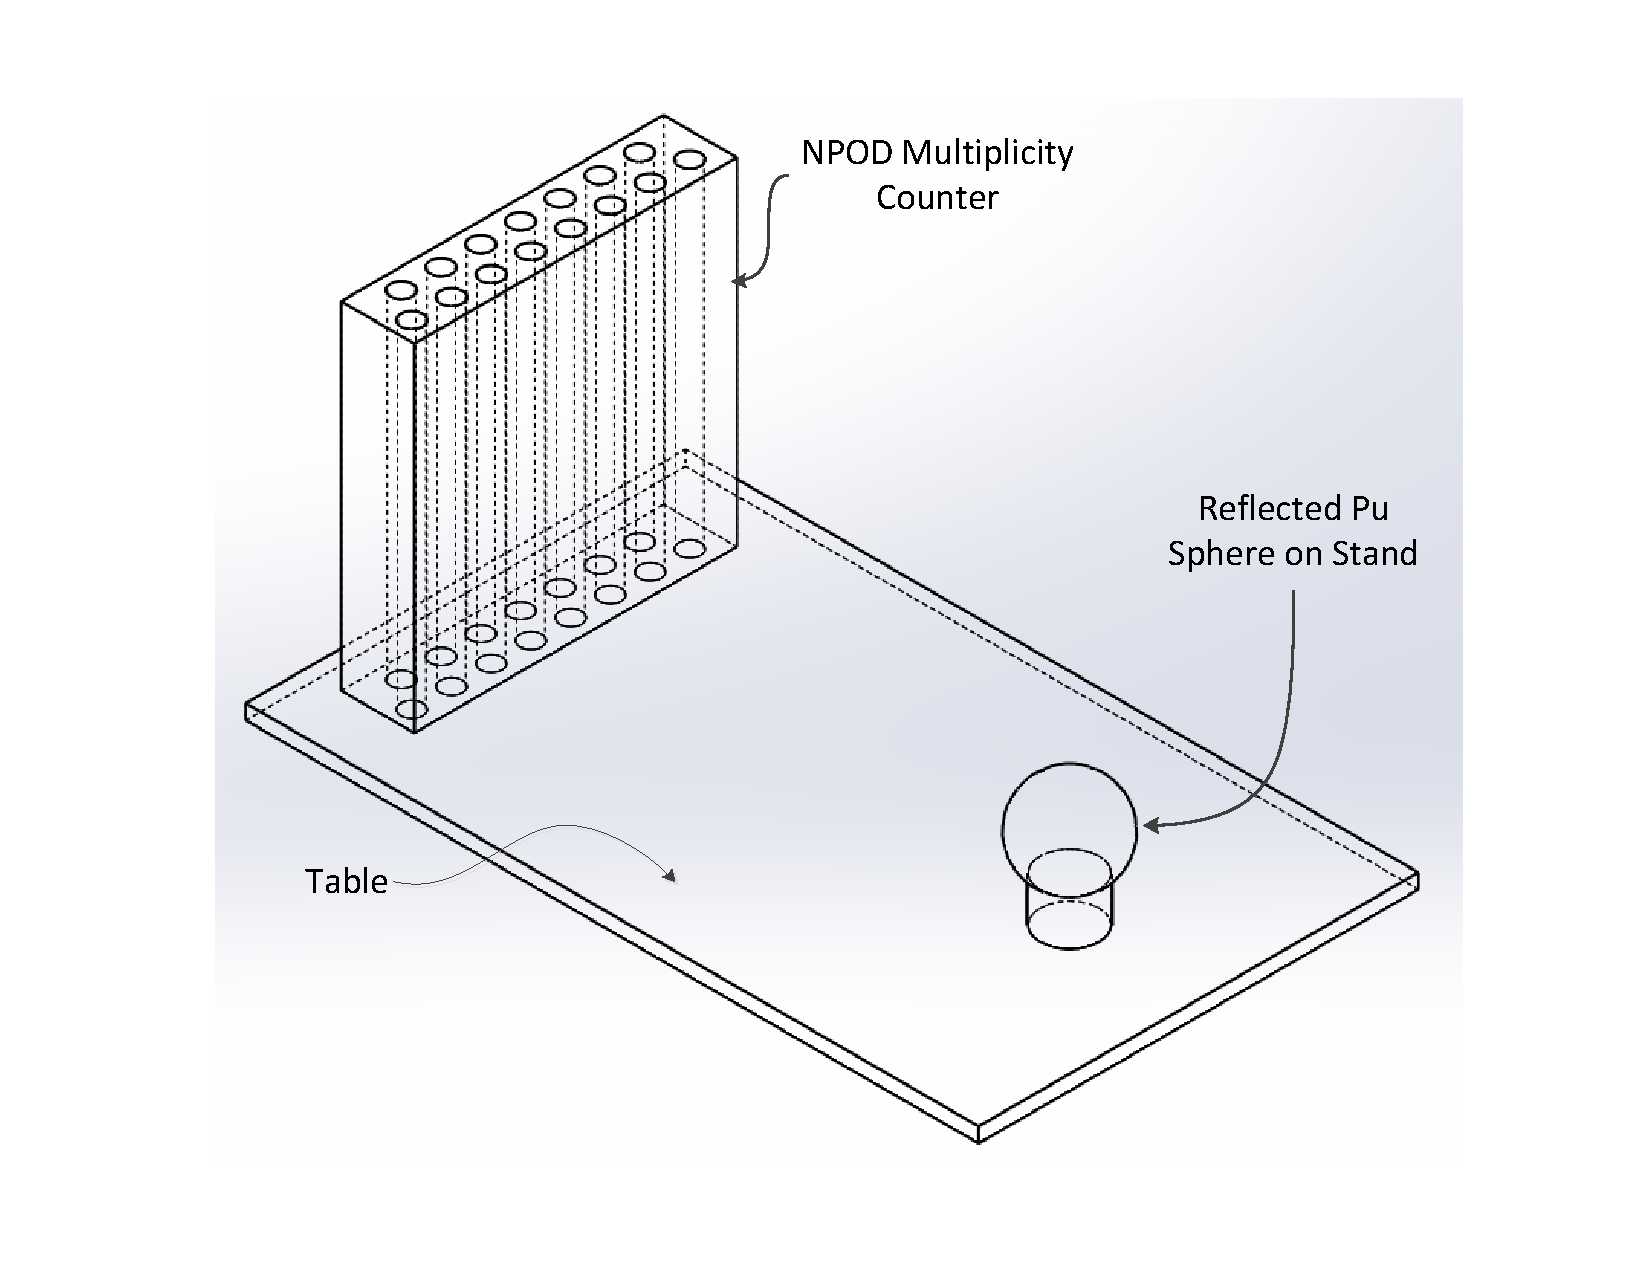
\includegraphics[trim=1.0in 0.70in 0.8in 0.50in,clip,width=1.19\textwidth]{multiplicity_experiment.pdf} \\
    {\fontsize{7pt}{6pt}\selectfont  *Not to scale}
\end{center}
\end{figure}
\end{minipage}
\begin{minipage}{0.54\linewidth}
    {\addtolength\leftmargini{-0.5in}
     \addtolength\leftmarginii{-0.2in}
     \addtolength\wideitemsep{0.1in}
\begin{itemize}
    \item[] Experimental Parameters
  \begin{itemize}
      \item 94\% \colb{\iso{Pu}{239}} sphere \vspace{-0.2in}
      \item 5 Different HDPE shells \\ \colG{From none to 3.0 cm HDPE}
  \end{itemize}
  \item[] Experiments repeated w/ \colb{\iso{Cf}{252}}
\end{itemize} 
}
\end{minipage}

\end{frame} 


\begin{frame}
    \frametitle{MCNP5 multiplicity simulations showed discrepancy \\ with experiments for
        Pu but not for \iso{Cf}{252}}
\begin{minipage}{0.41\textwidth}
\begin{figure}[ht!]
\begin{center}
	{
	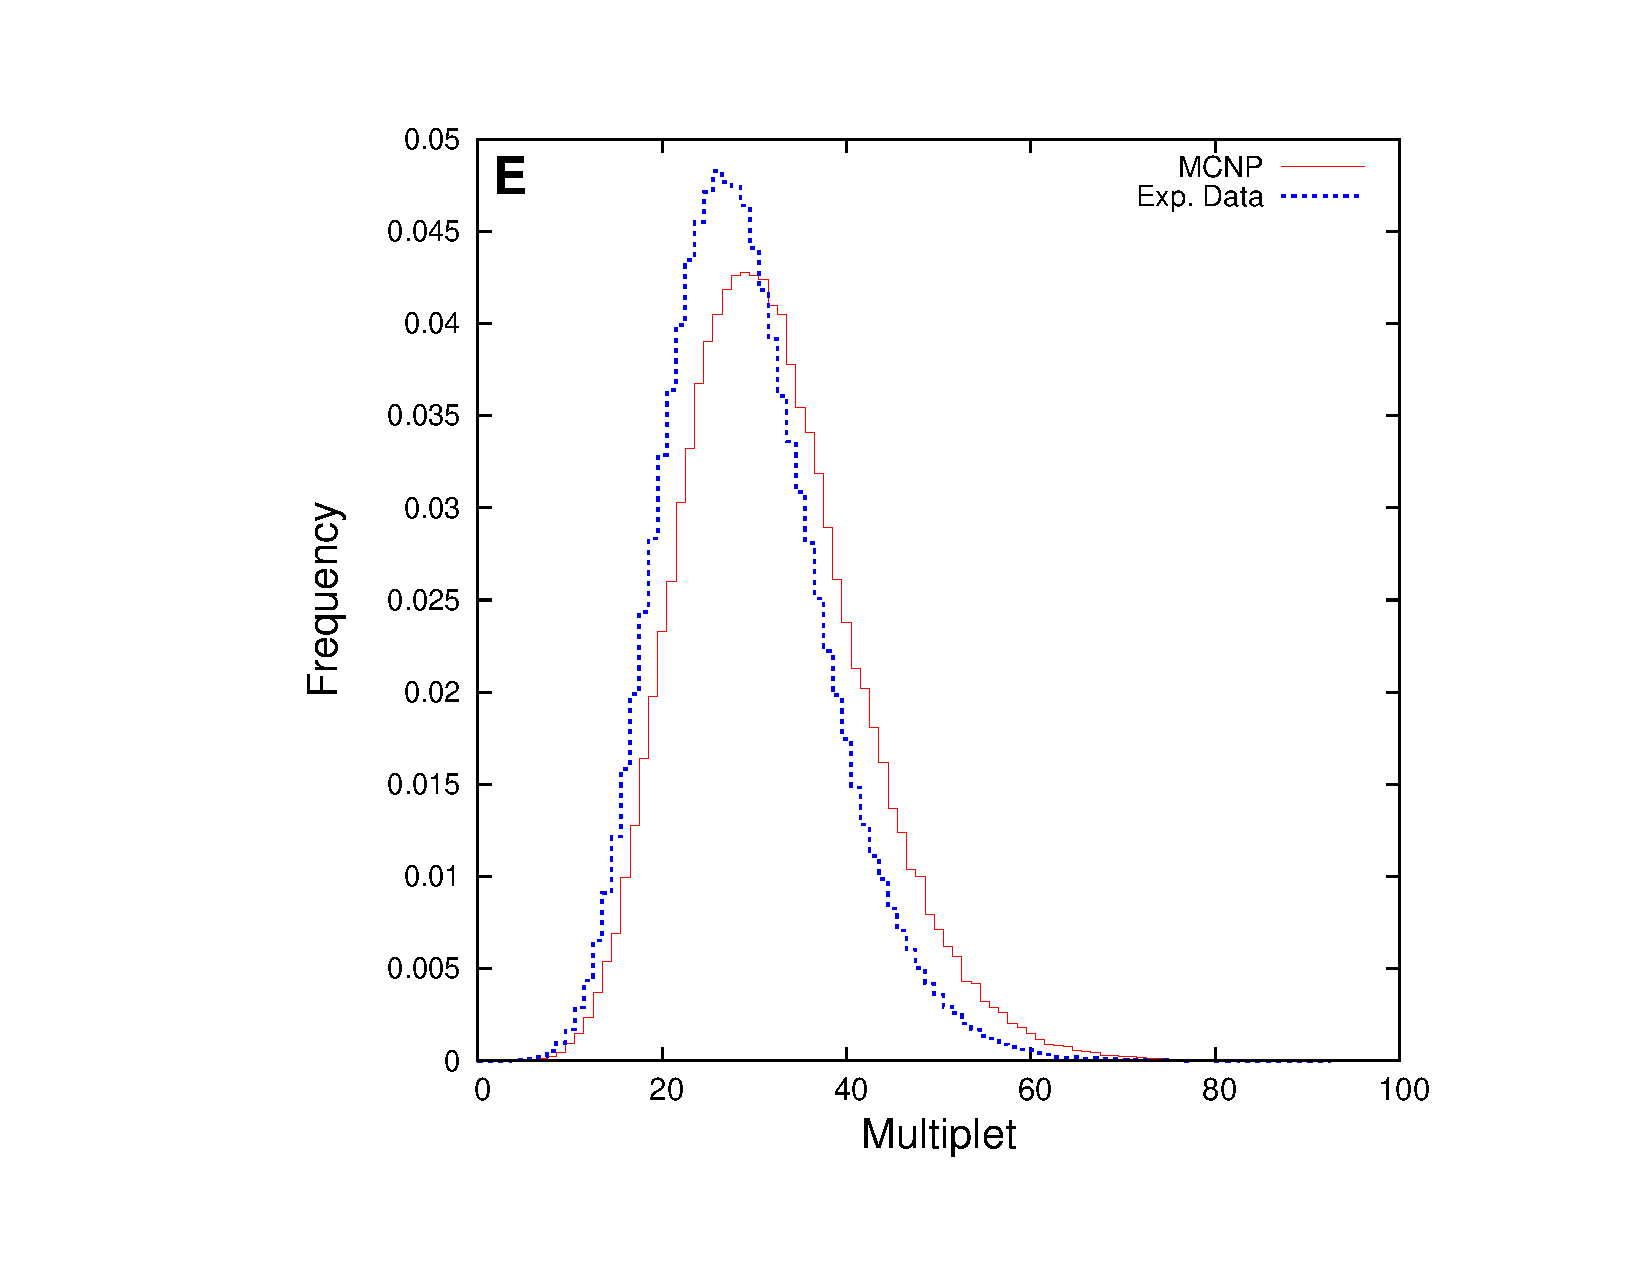
\includegraphics[trim= 2.00in 0.75in 1.450in 0.85in, clip, width=1.00\textwidth]{nubarFigures/trial_1_0_berp_3_0_2000.pdf} \\
	{\footnotesize Pu with 3.0-cm HDPE reflector} }
\end{center}
\end{figure} 
\begin{figure}[ht!]
\begin{center}
\end{center}
\end{figure} 

\end{minipage}
\begin{minipage}{0.56\textwidth}
    {\fontsize{10.8pt}{10pt}\selectfont
    \addtolength\leftmargini{-0.5in}
     \addtolength\leftmarginii{-0.2in}
     \addtolength\wideitemsep{0.1in}
\begin{itemize}
  \item[] Previous work by Mattingly [2010]
      \vspace{-0.1in}
  \begin{itemize}
      \item Caused by \textbf{\iso{Pu}{239}} \colb{nuclear data} 
	\vspace{-0.1505in}
	\item  Adjusted \colb{energy-integrated \nubar}	
	\end{itemize}
\item[]  In \textbf{ENDF-VII}, raised \nubar for \iso{Pu}{239} \\ \colG{to match \keff
    benchmarks}
    \vspace{0.1in}
  \begin{itemize}
 		\item \nubar is $\sim2\,\sigma$ \colr{above} measured data for $E < 1.5$ MeV 
	\end{itemize} 
\end{itemize} }
\end{minipage}
\end{frame} 
\begin{frame}
\frametitle{Can we reduce discrepancy in multiplicity distributions \\ without significantly
altering \keff?}
{\addtolength\leftmargini{-0.2in}
 \addtolength\wideitemsep{0.1in}
\begin{itemize}
    \item[] Perform energy-\colb{dependent} perturbations of $\overline{\nu}(E)$  in
        \iso{Pu}{239} \\ \colG{Random samples drawn from ENDF-VII.1 covariance data}
    \item[] Compare experimental and simulated multiplicity dist. 
            \\ \colG{and a $\keff$ benchmark (Jezebel)}
        \item[] Compare $\overline{\nu}(E)$ results to uniform shifts of
		microscopic cross sections 
	\end{itemize}	
}
\end{frame} 





%\section{Correlated Sampling}
%\subsection{Simulations of Multiplicity Experiments with Nuclear Data Perturbations}


%\section{Methodology}
%\subsection{Simulations of Multiplicity Experiments with Nuclear Data Perturbations}




\begin{frame}
\frametitle{We used LANL NDVV Python tools \\ to generate energy-dependent \nubar  samples}
{\addtolength\wideitemsep{0.2in}
\begin{enumerate}
	\item Generate a correlated sample of $\nubar(E)$ 
        \begin{itemize}\vspace{0.1in}
            \item {Assumed multivariate
                    Gaussian \\ \colG{ with group-averaged covariances}}
    \end{itemize}
  \item Modify continuous $\nubar(E)$ data in \textbf{ACE} file 
  \item Perform all MCNP simulations \\ \colG{with modified ACE data}
\end{enumerate} 
}
\end{frame} 



\begin{frame}
\frametitle{A cost function provides a measure \\ of inaccuracy for each data realization}
\begin{itemize}
	{
    \item[] \colb{Reduced} $\chi^2$ values for the 5 multiplicity experiments and criticality benchmark
        \begin{equation*} \hspace{0.4in}
		\begin{array}{c} 
            \displaystyle	\chi^2_{\text{red,mult,}m} = \frac{1}{N_{bins}-1}\sum_{i=1}^{N_{bins}}
	\frac{(P^{\textrm{exp}}_i - P^{\textrm{mcnp}}_i)^2}{\sigma^2(P^{\textrm{exp}}_i) + 
\sigma^2(P^{\textrm{mcnp}}_i)} 
		\end{array}
	\end{equation*} 
    \vspace{0.0in}
\item[] Equally weight $\chi^2$ values in a \colb{cost} function \\ \colG{A lower score indicatese
    higher accuracy}
	\begin{equation*}
        \boxed{\text{Cost} = \sum_{m=1}^5 \chi^2_{\text{red,mult,}m} + \chi^2_{\text{red,}\keff}}
	\end{equation*} 
}
\end{itemize}

\end{frame} 

%\begin{frame}
%\frametitle{Summary of Procedure}	
%\begin{itemize}
%	\item \colg{FOR} each \colb{trial} :
%	\begin{enumerate}
%		\item Generate a unique set of perturbed nuclear data
%		\item Run \textbf{MCNP5\_mult} simulations (5 multiplicity, \colb{JEZEBEL})
%		\item Produce multiplicity distributions
%		\item Compute $\chi^2_{red}$ values and cost
%	\end{enumerate} 
%	\item The \colb{lowest} cost is the most accurate trial
%\end{itemize}
%\end{frame} 


%\section{Results}
%\subsection{Simulations of Multiplicity Experiments with Nuclear Data Perturbations}

\begin{frame}
 \frametitle{Multiplicity and $\keff$ simulations were performed \\ for 500 unique realizations  of \nubar data}
\begin{center}
\resizebox{!}{0.5in}{
 \begin{tabular}{ccc}
	 \hline {Trial} & {Cost} & {$\chi^2_{\,{k}_{\mathrm{eff}}}$} 
\\ \hline
\nubar -1.14\%	&	164.24	&		33.66	\\	
\textbf{303}	&	\textbf{197.07}	&	\textbf{4.18}	\\	
%243	&	264.3	&	261.33	&	2.97	\\	
\colg{{55}}	&	267.9	&	\colg{0.01}	\\	
Original	&	426.86	&	0.27	\\	\hline
\end{tabular}
}
\end{center}
\begin{itemize}
    \item[]{MCNP criticality test suite performed for best data}
        \\ \colG{which includes 39 criticality benchmarks w/ \iso{Pu}{239}}:
\end{itemize}
	\begin{center}
\vspace{0.01in}
\resizebox{!}{0.50in}{
 \begin{tabular}{cc}
    \hline {Trial} & {$RMSD$} \\ \hline
\nubar -1.14\% & 1.23\% \\	
\colb{303} & \colb{0.51\%}	 \\
Original	&	0.49\% \\	\hline
\end{tabular}
}
\end{center}
\end{frame} 


\begin{frame}
\frametitle{Energy-dependent \nubar perturbations   \\ improved all 5 multiplicity
distributions}
\begin{itemize}
    \item Plots for best data realization and 3.0 cm HDPE case
\end{itemize}
\begin{center}
$\begin{array}{cc} \textbf{Original \nubar Data} & \hspace{0.13in}\textbf{Trial 303: Lowest Cost} \\
   \hspace{-0.25in}
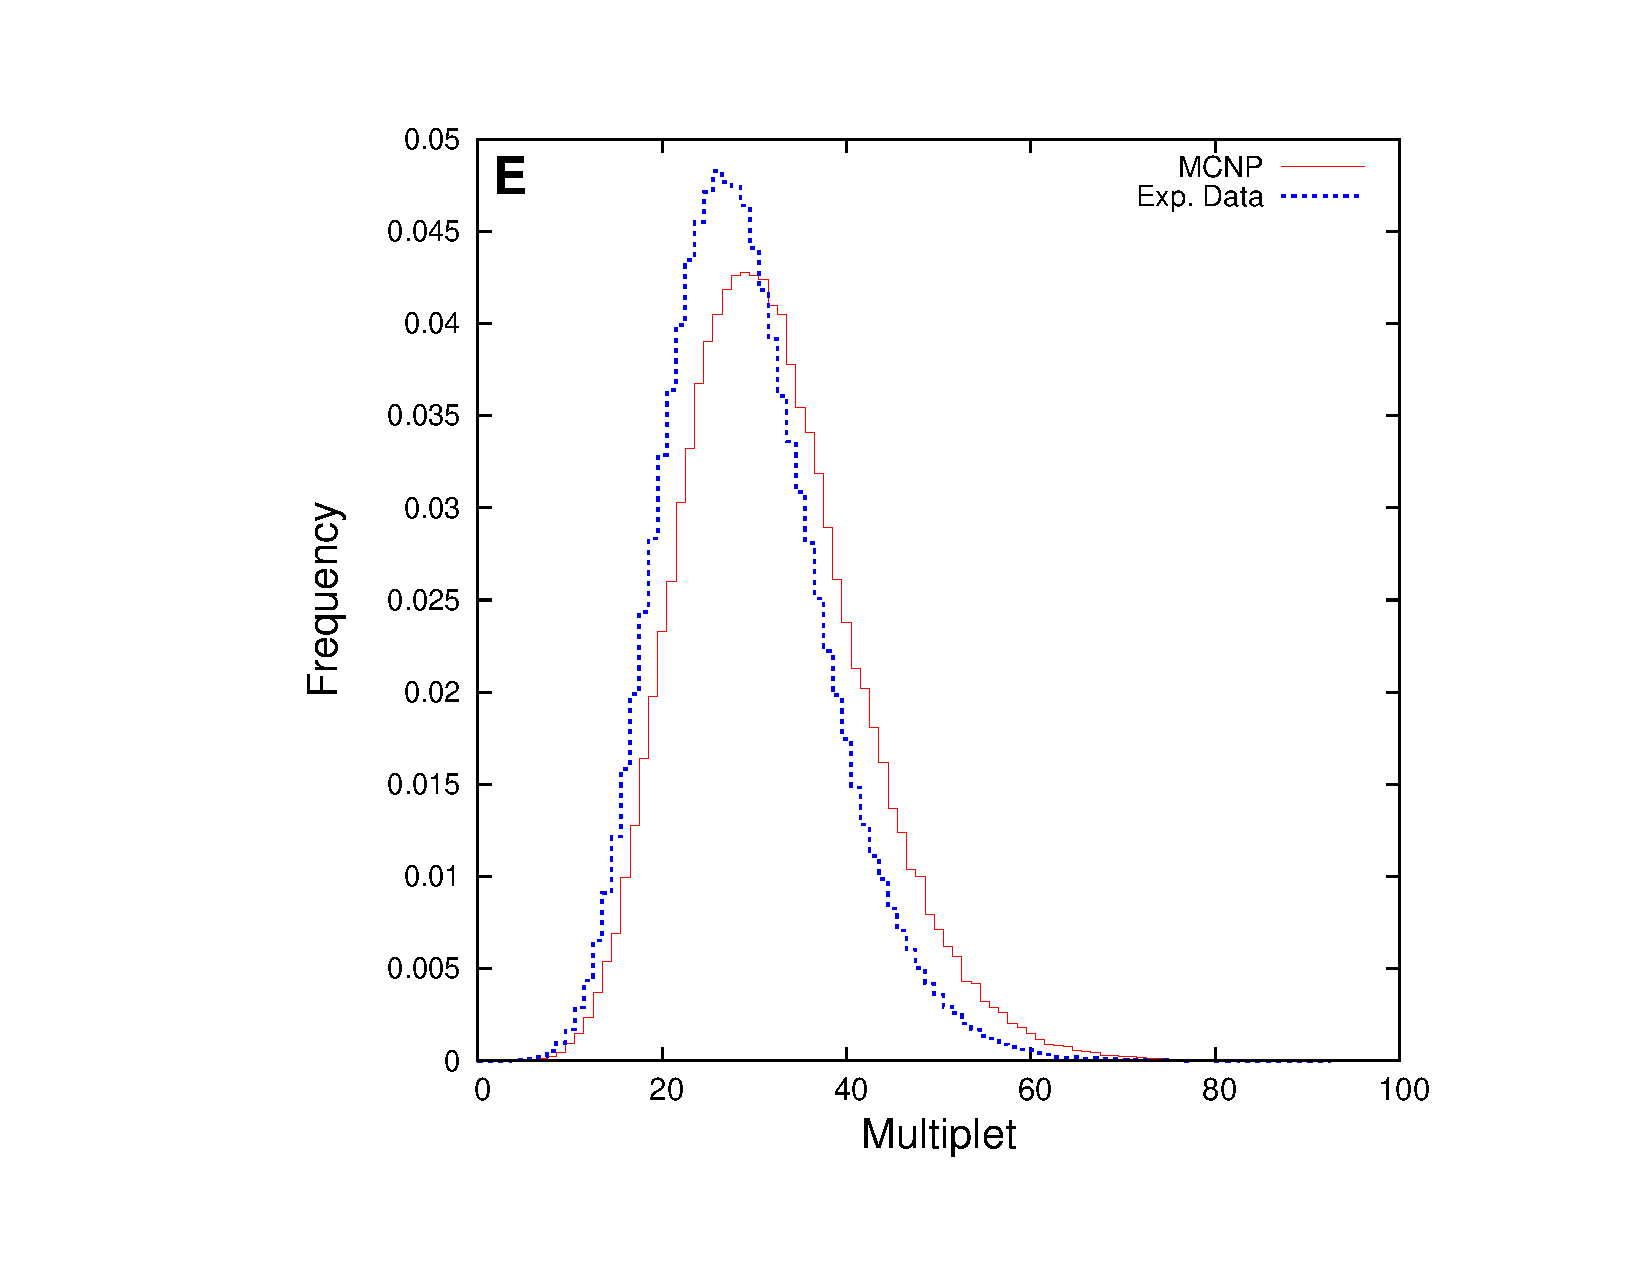
\includegraphics[trim= 1.0in 0.75in 1.0in 0.75in, clip, width=0.5\textwidth]{nubarFigures/trial_1_0_berp_3_0_2000.pdf} &
\hspace{-0.2in}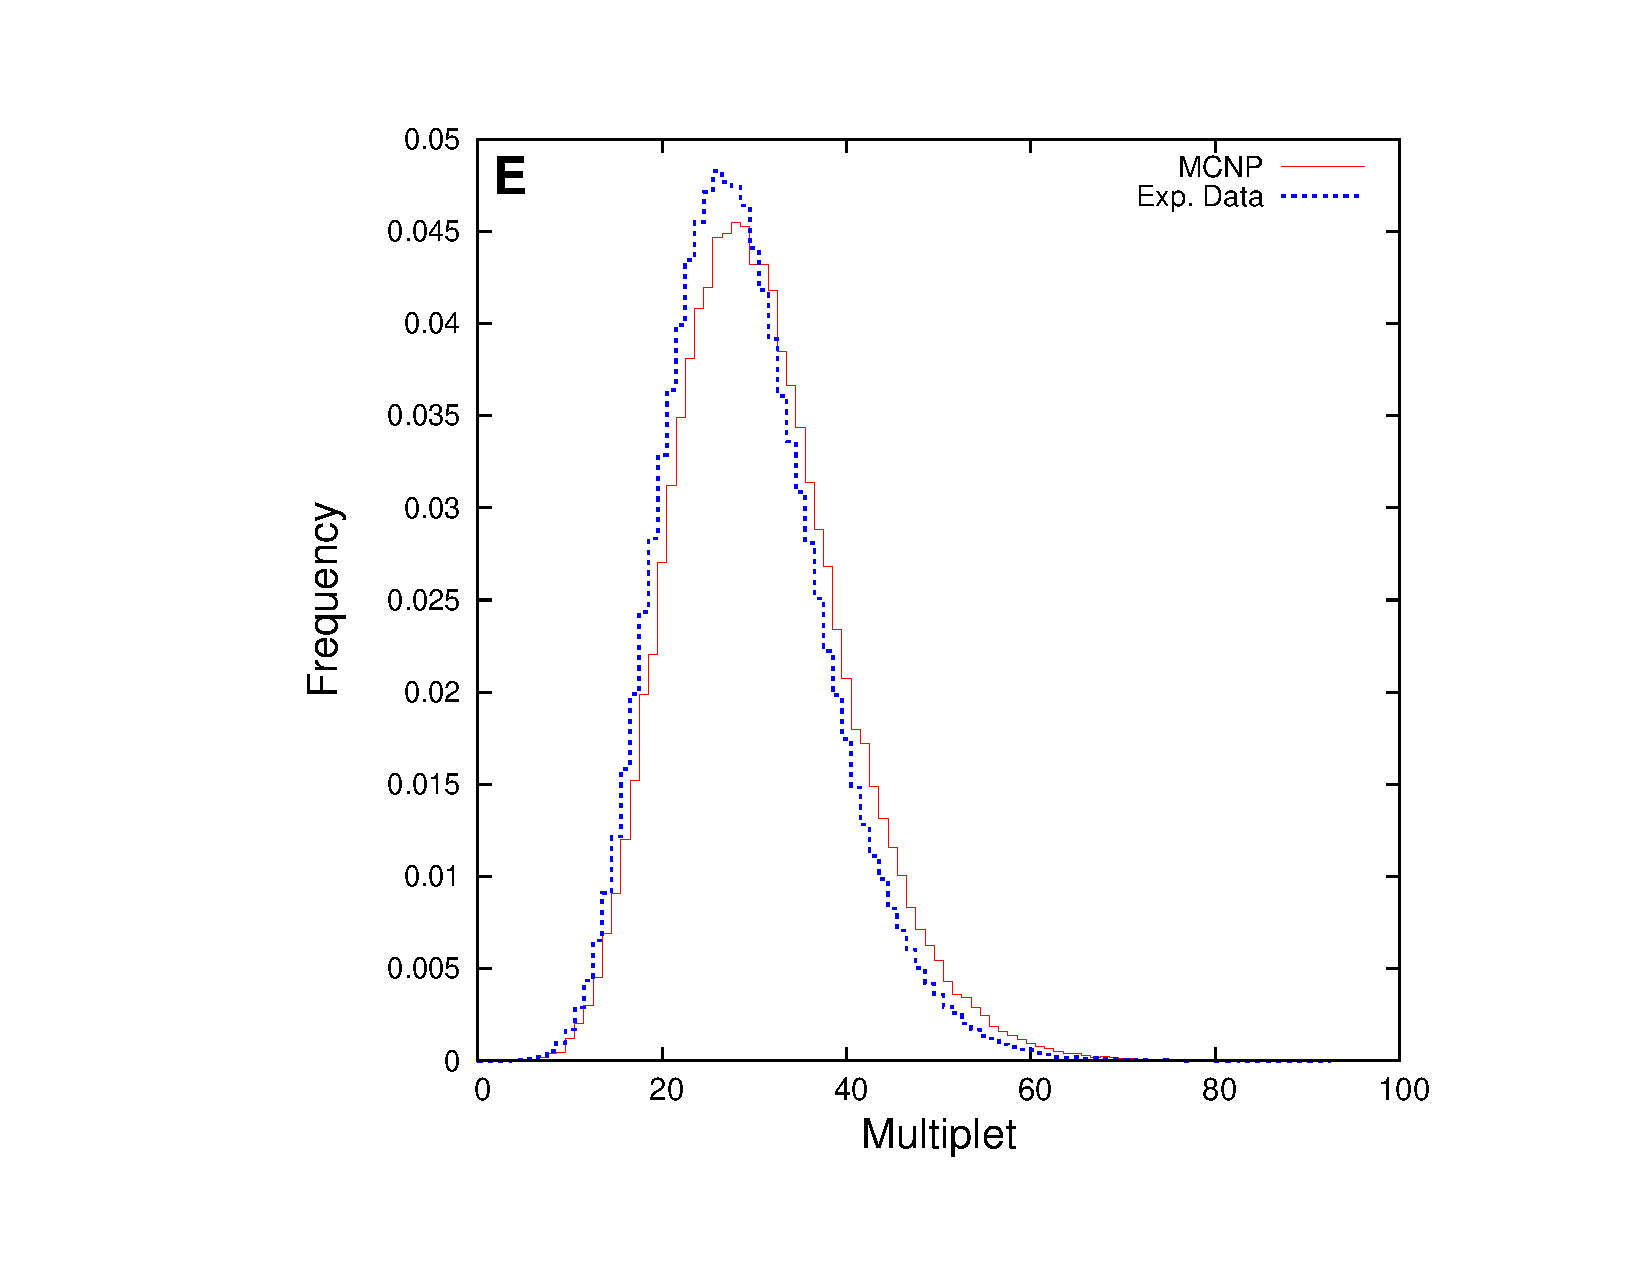
\includegraphics[trim=1.0in 0.75in  1.0in  0.75in, clip, width=0.5\textwidth]{nubarFigures/trial_303_berp_3_0_2000.pdf} \\
\end{array}$
\begin{itemize} 
	\item Best data set reduced \colb{bias} in {1$^{\text{st}}$} and {2$^{\text{nd}}$} moments, averaged over all 5 simulations, by \colb{$\sim35\%$}
\end{itemize}
\end{center}
\end{frame}


\logo{}

%\begin{frame}
%\frametitle{Capture Cross Section -- \coly{3.0 cm HDPE reflector}}
%{\small
%\begin{itemize} \vspace{-0.2in}
%	\item Adjust \colb{total cross section} ($\sigma_t$) to compensate for change in $\sigma_c$
%
%	\end{itemize} }
%	
%\begin{center}
%$\begin{array}{cc} \textbf{Original \sa Data} & \hspace{0.13in} {\sigma_c} \textbf{ increased 16\%} \\
%   \hspace{-0.25in}
%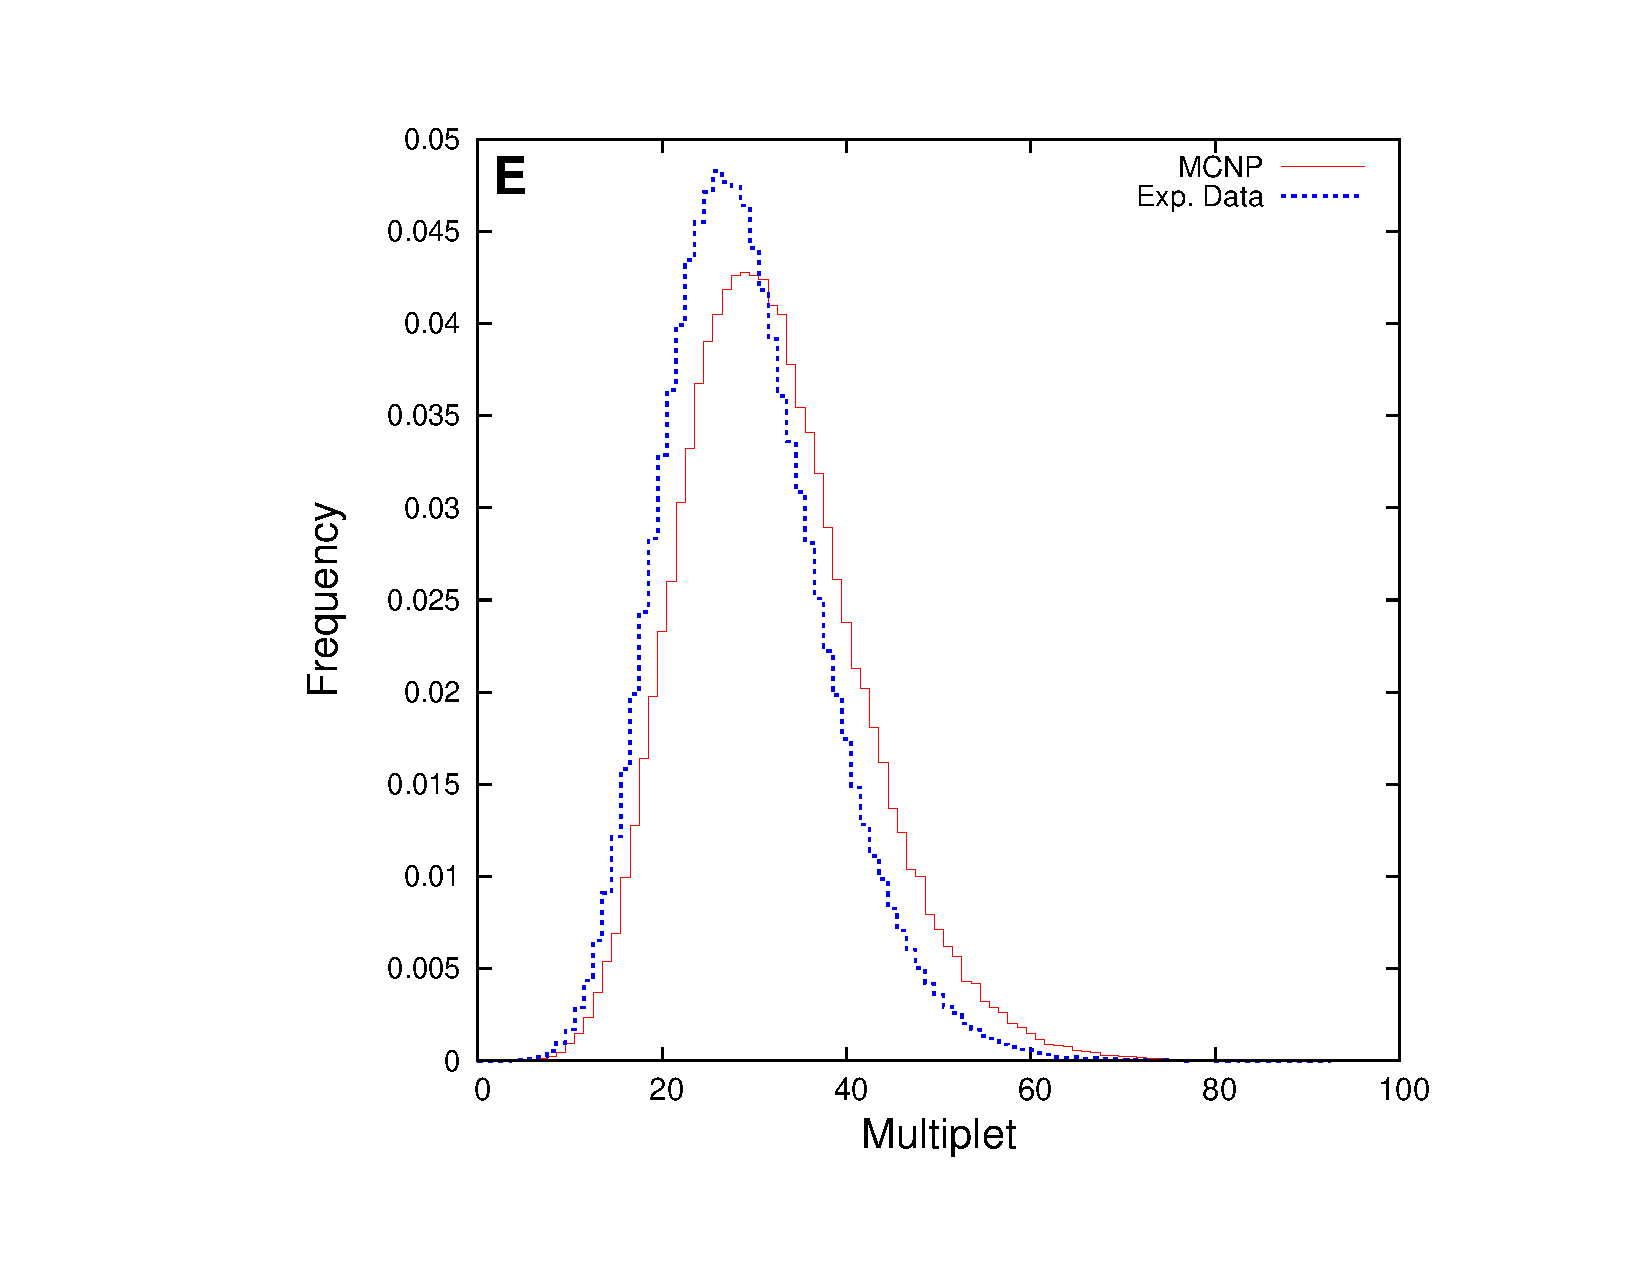
\includegraphics[trim= 1.0in 0.75in 1.0in 0.75in, clip, width=0.5\textwidth]{nubarFigures/trial_1_0_berp_3_0_2000.pdf} &
%\hspace{-0.2in}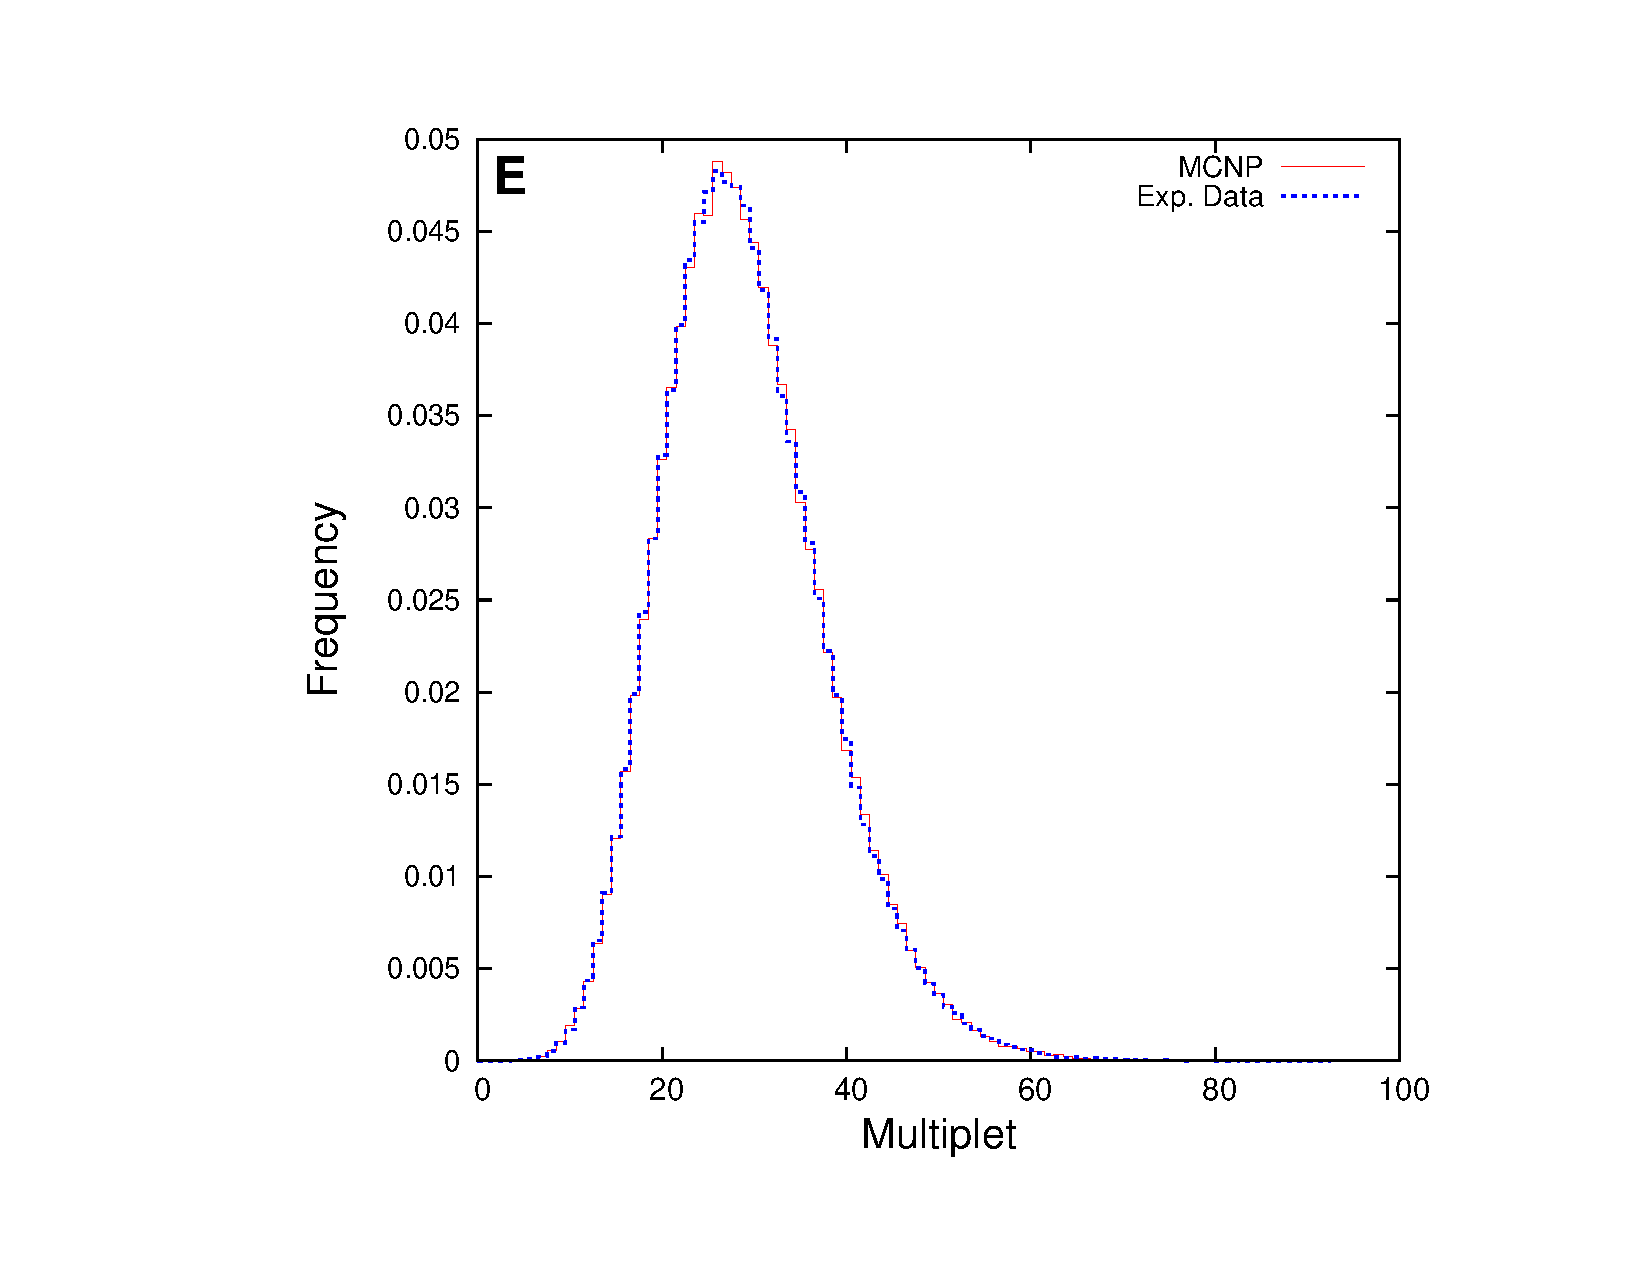
\includegraphics[trim=1.0in 0.75in  1.0in  0.75in, clip, width=0.5\textwidth]{capFigures/trial_16_0_berp_3_0_2000.pdf} \\
%\end{array}$
%\begin{itemize} 
%	\item Correction is \colr{less} for other experiments, and $\# s(\sigma_c) = \colr{7\;\sigma}$
%\end{itemize}
%\end{center}
%\end{frame}


\begin{frame}
    \frametitle{Adjusting the fission cross section \textbf{uniformly} \\ showed good correction to multiplicity
simulations}
\begin{center}
$\begin{array}{cc} \textbf{Original \sfiss Data} & \hspace{0.13in}\textbf{\sfiss decreased
    1.5\%} \\[6pt]
   \hspace{-0.25in}
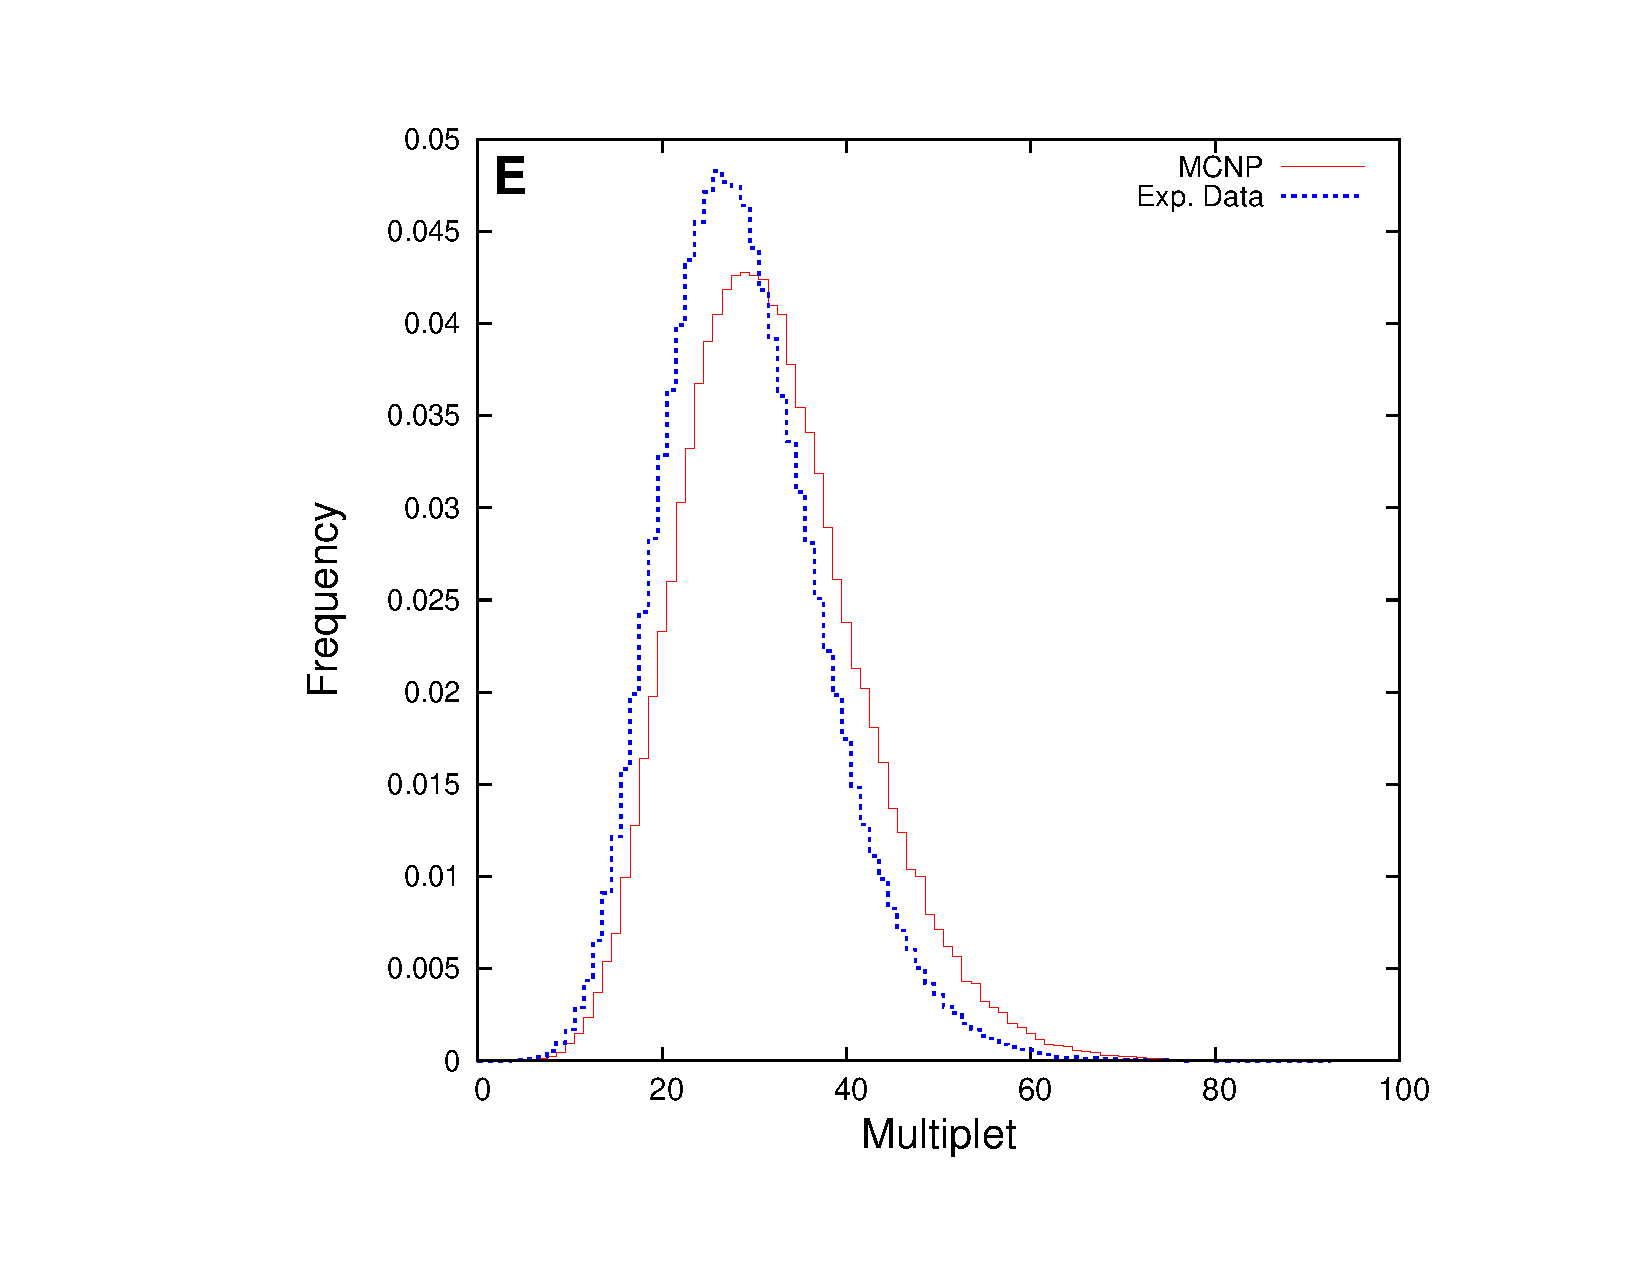
\includegraphics[trim= 1.0in 0.75in 1.0in 0.75in, clip, width=0.5\textwidth]{nubarFigures/trial_1_0_berp_3_0_2000.pdf} &
\hspace{-0.2in}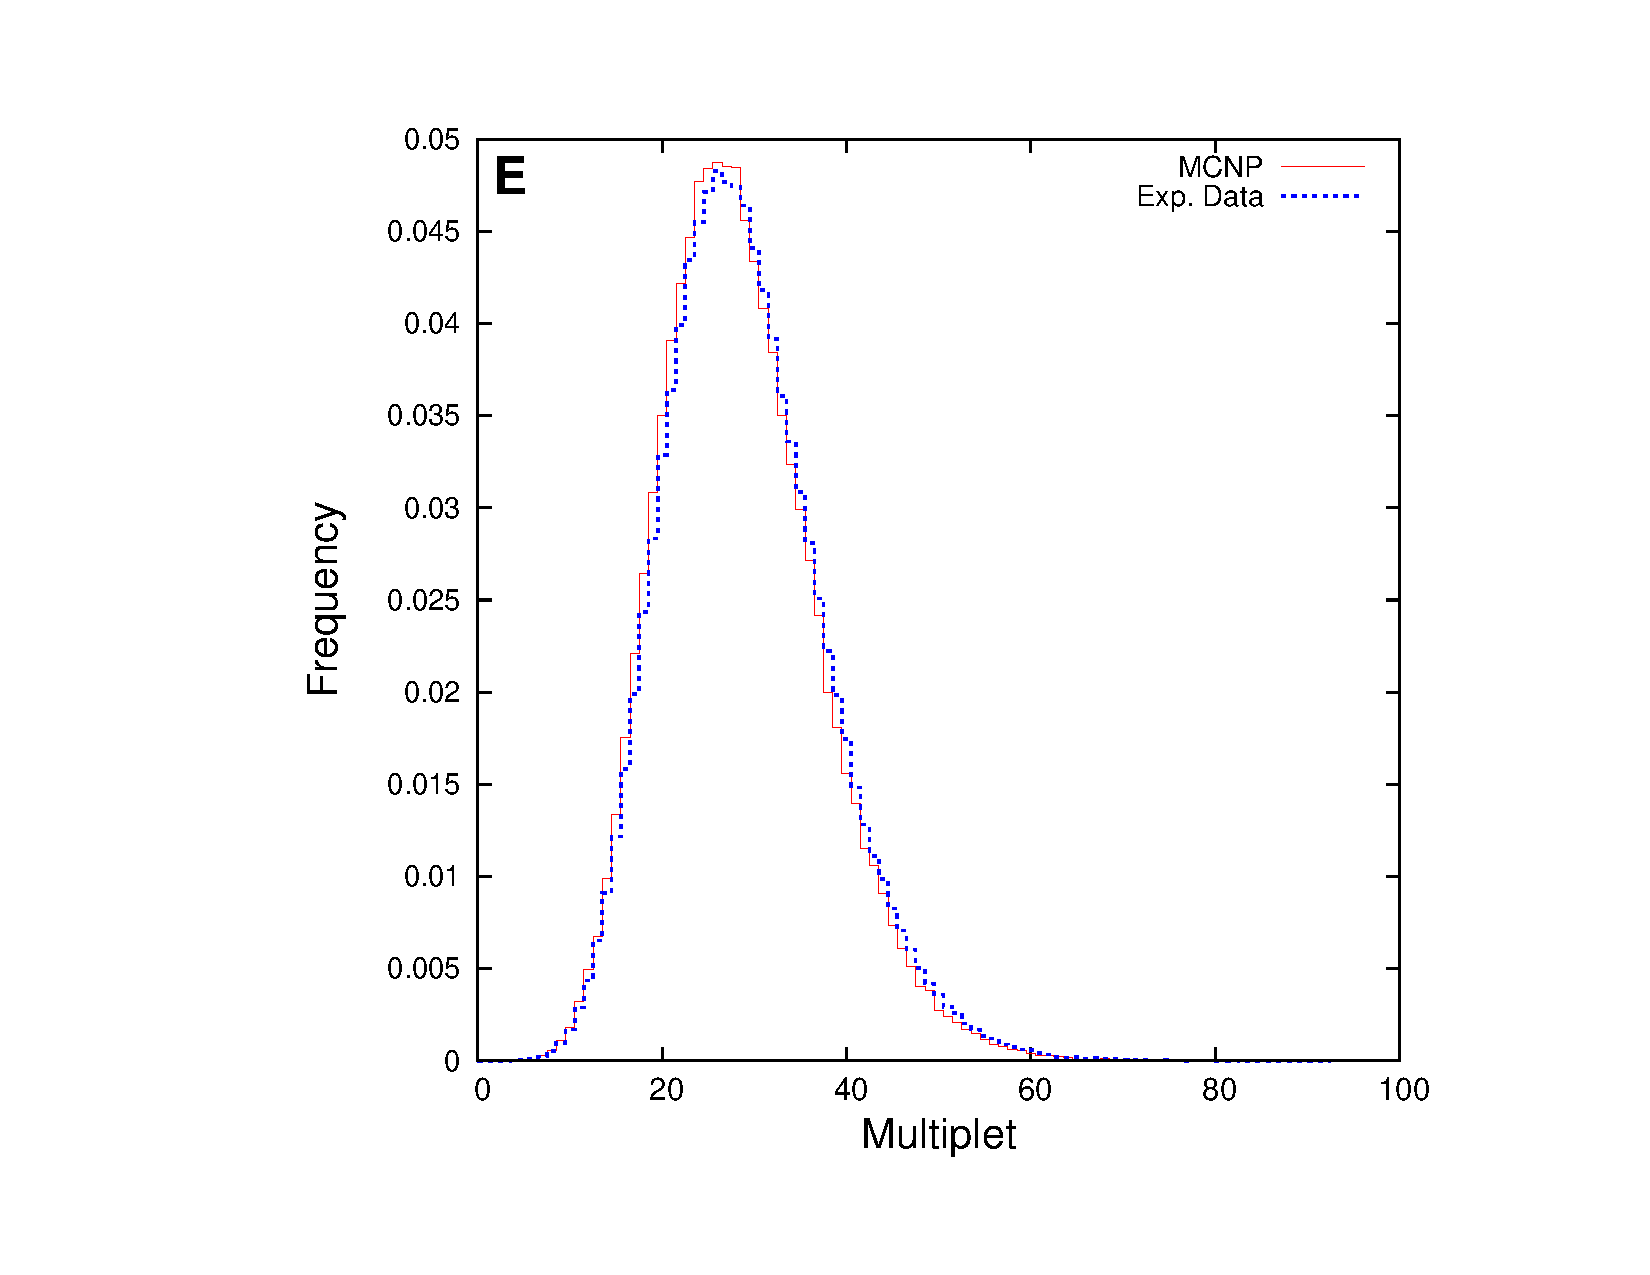
\includegraphics[trim=1.0in 0.75in  1.0in  0.75in, clip, width=0.5\textwidth]{capFigures/trial_-1_5_berp_3_0_2000.pdf} \\
\end{array}$
\end{center}
\begin{itemize} \vspace{-0.1in} 
  \item High accuracy for all simulations: $\displaystyle \sum_{i=1}^5 \chi^2_{red,mult,m} = \colb{14.6}$
      \vspace{-0.2in}
  \item \keff is \textbf{not preserved:} $\chi^2_{\keff} = 22.6$
\end{itemize} 
\end{frame}






%\section{Conclusions}
%\subsection{Simulations of Multiplicity Experiments with Nuclear Data Perturbations}
\begin{frame}
\frametitle{Simulations of Multiplicity Experiments \\ with Nuclear Data Perturbations}
	\vspace{-0.2in}
\begin{itemize}
    \item[] Energy-dependent \nubar perturbations \colb{reduced inaccuracies} in multiplicity while \colb{preserving} \keff
      \begin{itemize}\vspace{0.1in}
		\item Majority of cross-correlation terms $\mathcal{O}(10^{-4})$ or less
            \vspace{-0.1in}
        \item $\sigma_f$ may need more investigation
            \\ \colG{not sensitive to capture cross section}
	  \end{itemize}
      \item[] Subcritical simulations should be considered \\ in validation of nuclear data
      \item[] Covariance sampling methodology for nuclear data was developed and demonstrated
	\begin{itemize}
	 	\item Ideally sample all cross sections and \nubar simultaneously 

\end{itemize} 
\end{itemize}
\end{frame} 


\author{S.R. Bolding\inst{1}, \and C.J. Solomon\inst{2}}
\date{4 August 2016}
\begin{frame}
\vspace{-0.2in}
\centering
\maketitle

\end{frame} 

























\date{}
\title{Backup Slides}
\begin{frame}
    \vspace{-0.21in}
    \titlepage \vspace{-0.2113in}
\end{frame}

\appendix
\newcounter{finalframe}
\setcounter{finalframe}{\value{framenumber}}

\title{Backup Slides}
\author{}
\date{}

\begin{frame}
    \frametitle{Exponential convergence can be maintained if the LDFE mesh resolves the solution reasonably}
    \begin{columns}
    \begin{column}{0.5\textwidth}
        \vspace{0pt}
  \centering
    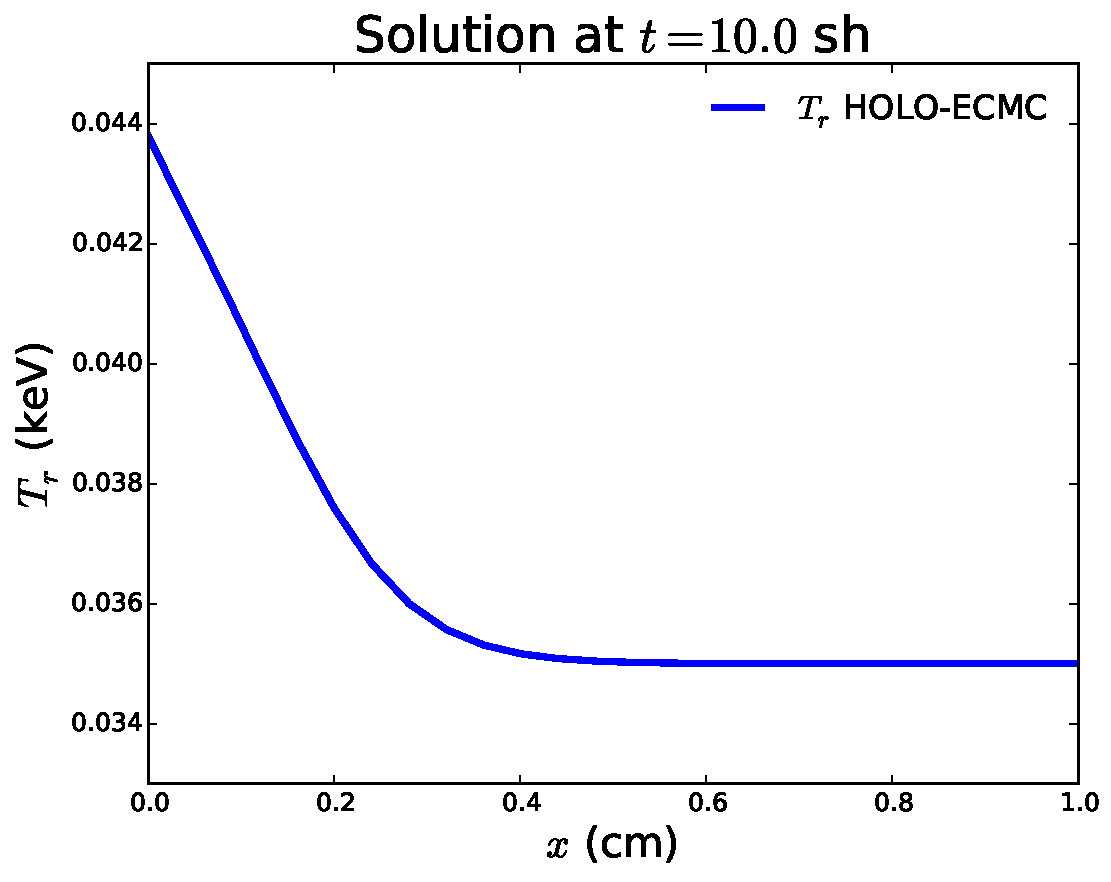
\includegraphics[width=\linewidth]{heated_marshak_new.pdf}
    \end{column}
    \begin{column}{0.5\textwidth}
        \vspace{0pt}
        \centering
        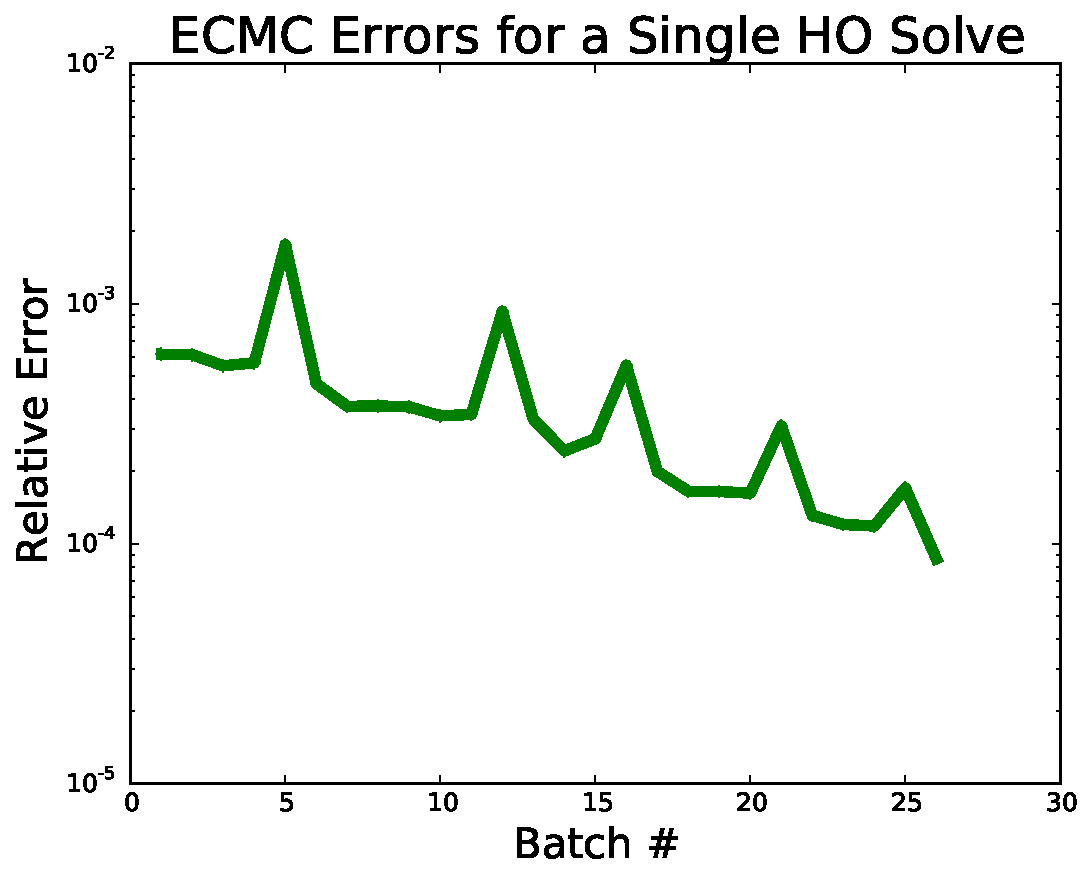
\includegraphics[width=\linewidth]{errors.pdf}
    \end{column}
\end{columns}
\end{frame}

\begin{frame}
    \frametitle{We can close equations with HO angular information \\ and a 
        linear-discontinuous (LD) spatial
    discretization}
    \begin{columns}
        \begin{column}{0.2\linewidth}
    \begin{centering}
        \begin{tikzpicture}[scale=0.62, every node/.style={transform shape}]
            \draw (1.0,2.125) node[fill,circle,inner sep=0pt,minimum
            size=4.2pt] {};
            \draw (1.0,0.4) -- (1.0,0.6) node[below, pos=0.4] {$x_{i-1/2}$};
            \draw (5.90,0.4) -- (5.90,0.6) node[below, pos=0.4] {$x_{i+1/2}$};
            \node at (5.6,4.1) {$T_{i,R}^4$};
            \node at (1.2,2.7) {$T_{i,L}^4$};
            \draw [thick] (1.0,0.5) -- (5.9,0.5) node[anchor=north west] {};
            \draw (1.0,2.125) -- (5.90,3.70);
            \draw (5.9,3.70) node[fill,circle,inner sep=0pt,minimum
            size=4.2pt] {};
        \end{tikzpicture}
        \vspace{0.1in}
        \begin{tikzpicture}[scale=0.58, every node/.style={transform shape}]
            \hspace{-0.13in}
            \draw [Gray,thick,dashed] (-1.2,-1.) -- (6.25,-1.);
        \end{tikzpicture}
        \begin{tikzpicture}[scale=0.62, every node/.style={transform shape}]
            \draw (1.0,4.0) node[fill,circle,inner sep=0pt,minimum
            size=4.2pt] {};
            \filldraw[color=black, fill=white] (1,2.1250) circle (2.1pt);
            \draw [->] (1.6,4.25) -- (2.4,4.25) node[anchor=west] {$\mu$};
            \draw (1.0,0.4) -- (1.0,0.6) node[below, pos=0.4] {$x_{i-1/2}$};
            \draw (5.90,0.4) -- (5.90,0.6) node[below, pos=0.4] {$x_{i+1/2}$};
            \node at (4.6,3.70) {$\phi^+(x)$};
            \draw [thick] (1.0,0.5) -- (5.9,0.5) node[anchor=north west] {};
            \draw (1.0,2.125) -- (5.90,3.50);
            \draw (5.9,3.50) node[fill,circle,inner sep=0pt,minimum
            size=4.2pt] {};
        \end{tikzpicture}
    \end{centering}
\end{column}
\begin{column}{0.75\linewidth}
    \addtolength{\wideitemsep}{0.11in}
    \begin{enumerate}
        \item Assume $T(x)$ and $T^4(x)$ are LD 
        \item A lagged \colb{ $\tilde{I}_{\text{HO}}^{n+1}$} is used \\ to evaluate
        consistency terms 
        \item Eliminate $\phi_{i+1/2}^\pm$ with LD closure
            \colG{preserving equi. diff. limit}
            \begin{center}{\textcolor{Gray}{%
                    \fbox{ {\color{black} $\displaystyle  
      \phi_{i+1/2}^+ = 2\mom{\phi}_{R,i}^+ - \mom{\phi}_{L,i}^+$}}}}
            \end{center}
       \item Global system solved with Newton's method and lagged \textbf{implicit
           opacities}\\ \colG{Energy is always conserved}
       \end{enumerate}
    \end{column}
\end{columns}
\end{frame}

\begin{frame}
    \frametitle{We need a way to resolve issues when the LDFE representation of the intensity is
        negative}
    {\addtolength\wideitemsep{5pt}
    \begin{itemize}
        \item[] Negative intensities can occur in optically thick cells \\
            \colG{Mesh refinement is of minimal use}
        \item[] $\tilde I_{HO}(x,\mu)$ must be positive for consistency terms \\
            \colG{to produce a physical, stable LO solution}
         \item[] Independent fix up for LO solution
             \colG{\\E.g., lumping or preserving balance with floored $\phi(x)$}
    \end{itemize}
}

\end{frame}




\begin{frame}
    \frametitle{Can add source $\delta$ to produce a positive projection $\tilde I_{pos}$ 
        such that $\tilde I_{pos}$ satisfies the
    latest residual equation}
    {\addtolength\wideitemsep{0.1in}
    \begin{itemize} 
        \item[] Produce $\tilde I_{\text{pos}}$ by scaling $x-\mu$ moments equally,
            \\ \colG{to estimate source for the next iteration\vspace{0.1in}}
            \begin{tikzpicture}
                \hspace{-0.20771in}
            \node at (0,0) {$\!\begin{aligned}
                \B L \tilde I^{(m)}  &= q - r^{(m)} \\
                    \B L \tilde I_{\text{pos}}^{(m)} &= q - r^{(m)} + \colb{\delta^{(m+1)}}
            \end{aligned}$};
             \node at (2.73,0.1) [fill=Gray!50,shape=single arrow,text width=0.7cm,text
             height=0.00001cm,line width=0.01cm] {};
             \node at (5.62,0){$\!\begin{aligned}
                     \delta^{(m+1)} &= \B L \left(\tilde I^{(m)} - \tilde
             I_{\text{pos}}^{(m)}\right)  \\
             q &\rightarrow q + \delta^{(m+1)}
            \end{aligned}$};
            \end{tikzpicture}
        \item[] We can delay error stagnation
            \\ \colG{Investigating alternative positive projection of $I$}
    \end{itemize}
}
\end{frame}

\begin{frame}
    \frametitle{Solving LO System with Newton's Method}
    \begin{block}{}
    \begin{itemize}
        \item Linearization: $\displaystyle \u B(T^{n+1}) = \u B(T^*) + \left(T^{n+1} -
                T^*\right) \pderiv{\u B}{t}\bigg|_{t^*}$
        \vspace{-0.15in}
        \item Modified system
            \begin{gather*}
                \displaystyle \left[\B  D(\mu^\pm) - \sigma_a^*(1-f^*) \right]\underline
                \Phi^{n+1}  = f^* \u B(T^*) + \frac{ \underline \Phi^n}{c\Delta t} \\
                \boxed{\hat{ \B  D }\Phi^{n+1} = \underline Q}
            \end{gather*}
        \vspace{-0.07in}
        \begin{center}
         $\displaystyle f = \left( 1 + \sigma_a^*c \Delta t \frac{4aT^{*3}}{\rho
            c_v} \right)^{-1}$  \hspace{0.3in}
         $\displaystyle T_i^* = \frac{T^{*}_{L,i}+T^{*}_{R,i}}{2}$
     \end{center}
 \item Equation for $T^{n+1}$ based on linearization that is conservative
 \item Converge $T^{n+1}$ and $\mom{\phi}$ with Newton Iterations
 \end{itemize}
 \end{block}
\end{frame}


%\begin{frame}
%    \frametitle{We will use a linear doubly-discontinuous (LDD) trial space  to allow for a HO
%        spatial closure}
%    \begin{columns}
%        \begin{column}[t]{0.2\textwidth}
%            \vspace{0pt}
%    \begin{center}
%        \begin{tikzpicture}[scale=0.62, every node/.style={transform shape}]
%            \draw (1.0,4.0) node[fill,circle,inner sep=0pt,minimum
%            size=4.2pt] {};
%            \draw [->] (1.6,4.25) -- (2.4,4.25) node[anchor=west] {$\mu$};
%            \draw (1.0,0.4) -- (1.0,0.6) node[below, pos=0.4] {$x_{i-1/2}$};
%            \draw (5.90,0.4) -- (5.90,0.6) node[below, pos=0.4] {$x_{i+1/2}$};
%            \node at (3.6,3.06) {$\phi_{LO}^+(x)$};
%            \draw [thick] (1.0,0.5) -- (5.9,0.5) node[anchor=north west] {};
%            \filldraw[color=black, fill=white] (1,3.1250) circle (2.1pt);
%            \draw (1.0,3.125) -- (5.90,2.120);
%            \filldraw[color=cyan, fill=white] (5.9,2.120) circle (2.1pt);
%            \draw (5.9,3.0) node[cyan,fill,circle,inner sep=0pt,minimum size=4.2pt] {};
%        \end{tikzpicture}
%    \end{center}
%    \end{column}
%    \begin{column}[t]{0.8\textwidth}
%    \vspace{0pt}
%    \begin{itemize}
%        \item $\tilde I_{HO}(x,\mu)$ will be linear in $\mu$ along face \\
%    \colG{Error estimated with MC face tallies}
%        \vspace{0.1in}
%        \item In LO equations use LDD for $\phi^{\pm}$\\
%             \colG{The linear interior preserves the EDL}
%        \vspace{0.1in}
%        \item Parameterize LO spatial closure to eliminate outflow:
%            \begin{equation*}
%                \phi^{+}_{i+1/2} = \frac{3+\highlight{\gamma_{i,HO}^+}}{2} \mom{\phi}_{R,i}^+ +
%                \frac{\highlight{\gamma^+_{i,HO}} - 3}{2}
%                \mom{\phi}_{L,i}^+
%            \end{equation*}
%    \end{itemize}
%    \end{column}      
%    \end{columns}
%\end{frame}

\begin{frame}   
    \frametitle{The angular flux for the two material problem is difficult to resolve near
    $\mu=0$}
    \begin{figure}
        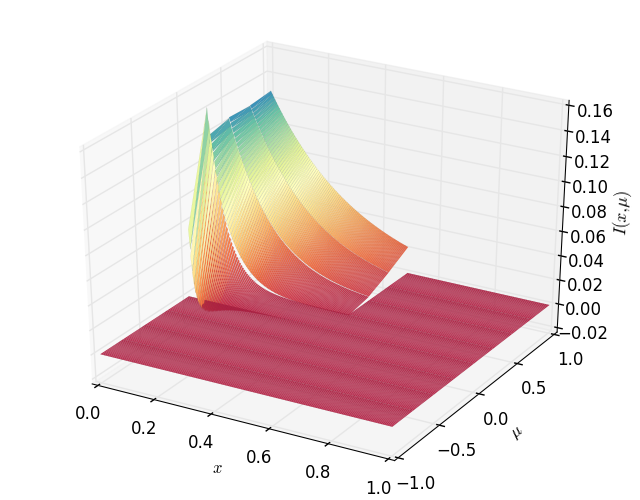
\includegraphics[width=0.57\textwidth]{ang_flux.png}
    \end{figure}
\end{frame}

%%%%%%%%%%%%%%%%%%%%%%%%%%%%%%%%%%%%%%%%%%%%%%%%%%%%%%%%%%%%%%%%%%%%%%%%%%%%%%%%%%%%%%%%%
\begin{frame}
    \frametitle{Two Material Problem, comparison in optically thin region}
    \begin{block}{}
        \begin{itemize}
            \item Plot of radiation temperature after 10 time steps
        \end{itemize}
    \end{block}
\begin{figure}
    \centering
    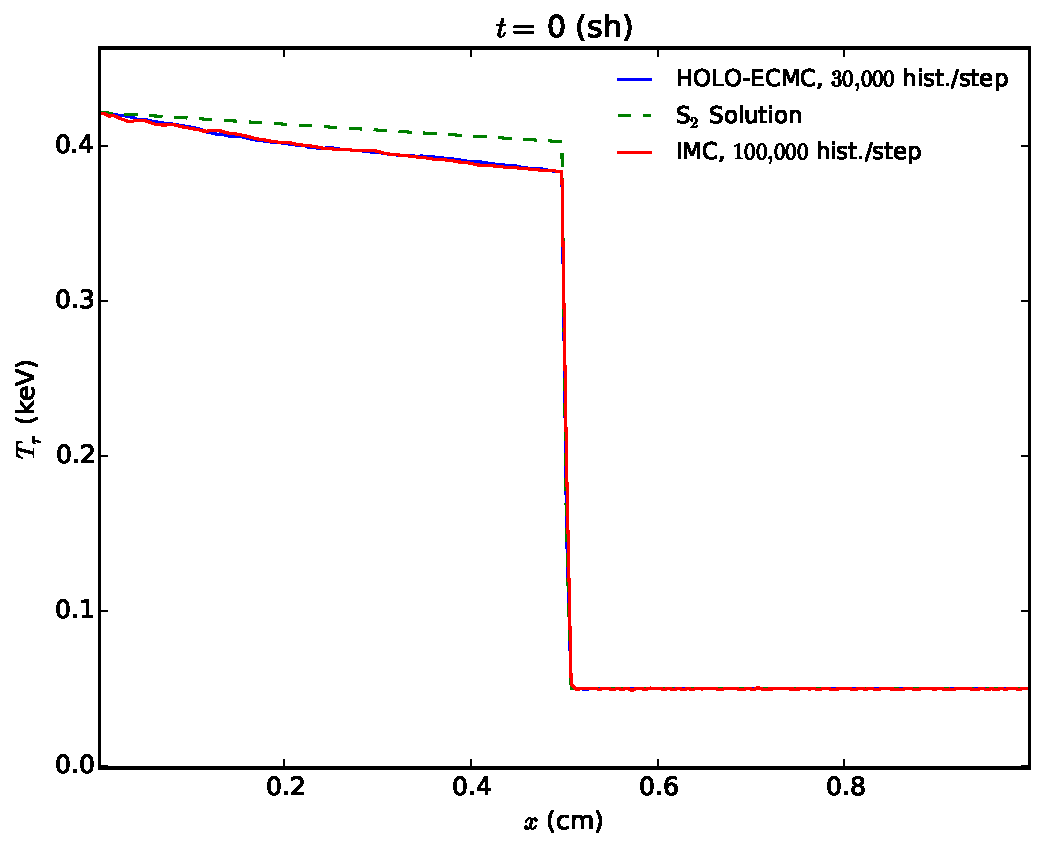
\includegraphics[width=0.5799\textwidth]{quick_compare.pdf}
\end{figure}

\end{frame}


\begin{frame}
    \frametitle{Backup slide with timing results}

\end{frame}



\begin{frame}
    \frametitle{Forming the LO System}
    \begin{itemize}
        \item Taking moments of TE yields \colb{4 equations}, per cell $i$, e.g.
\begin{multline}\label{lo_tran}
    -2{\mu}_{i-1/2}^{n+1,+} \phi_{i-1/2}^{n+1,+} + \cur {\mu}_{L,i}^{n+1,+}
  \mom{\phi}_{L,i}^{n+1,+}
  +  \cur\mu_{R,i}^{n+1,+}
  \mom{\phi}_{R,i}^{n+1,+} +  \\ \left(\sigma_t^{n+1}+\frac{1}{c \Delta t} \right) h_i 
  \mom{\phi}_{L,i}^{n+1,+} -  \frac{\sigma_s h_i}{2} \left( \mom{\phi}_{L,i}^{n+1,+} +
  \mom\phi_{L,i}^{n+1,-}\right) \\ = \frac{h_i}{2} \mom{\sigma_a^{n+1} a c T^{n+1,4}}_{L,i} +
  \frac{h_i}{c\Delta t}\mom{\phi}_{L,i}^{n,+},
\end{multline}
        \item Cell unknowns: $\mom{\phi}_{L,i}^{+}$, $\mom{\phi}_{R,i}^{+}$,
        $\mom{\phi}_{L,i}^{-}$, $\mom{\phi}_{R,i}^{-}$, $T_L$, $T_R$

    \item Need \colb{angular} consistency terms  and spatial closure
        (LD)
    \end{itemize}

\end{frame}

\begin{frame}
\frametitle{Neutron multiplicity distributions provide passive \\ multiplication
information about a fissionable system}
 \centering
 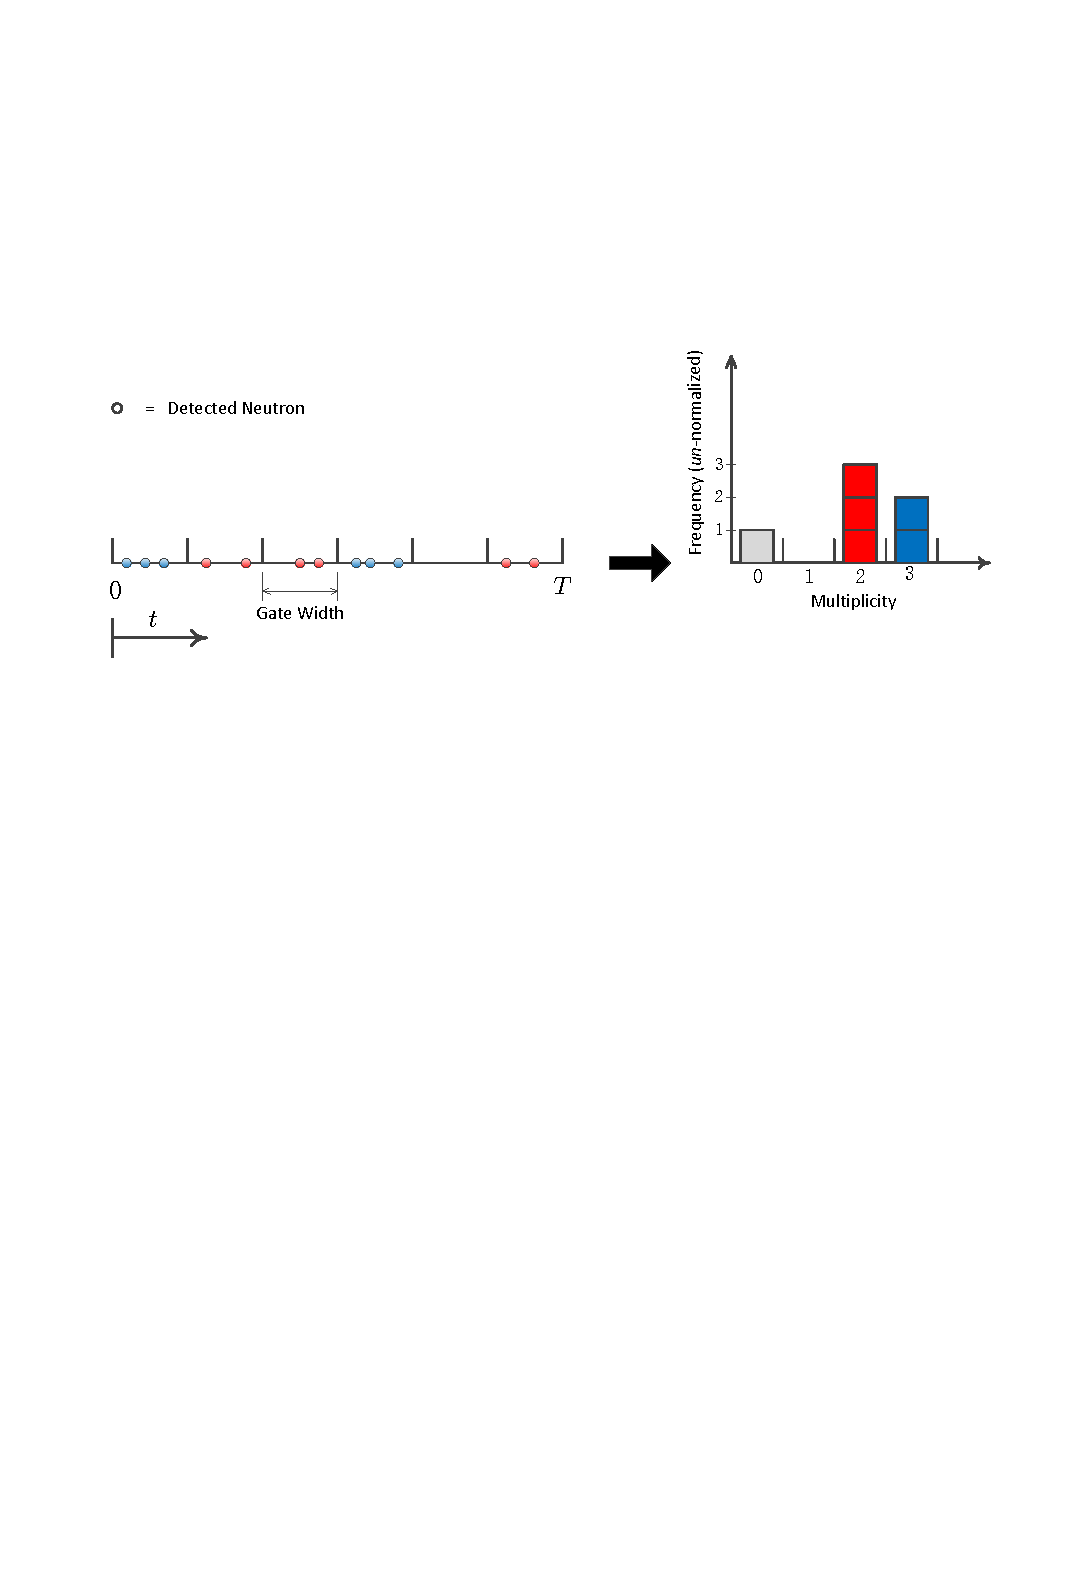
\includegraphics[trim=0.7in 6.075in 0.6in 2.0in,clip,width=1.0\textwidth]{neutron_hist.pdf}

\end{frame}




\begin{frame}
	\frametitle{Energy-\colb{Integrated} \nubar Shift -- {3.0 cm HDPE reflector}}
\begin{center}
$\begin{array}{cc} \textbf{Original \nubar Data} & \hspace{0.13in}\textbf{-1.14\% \nubar} Data\\
   \hspace{-0.25in}
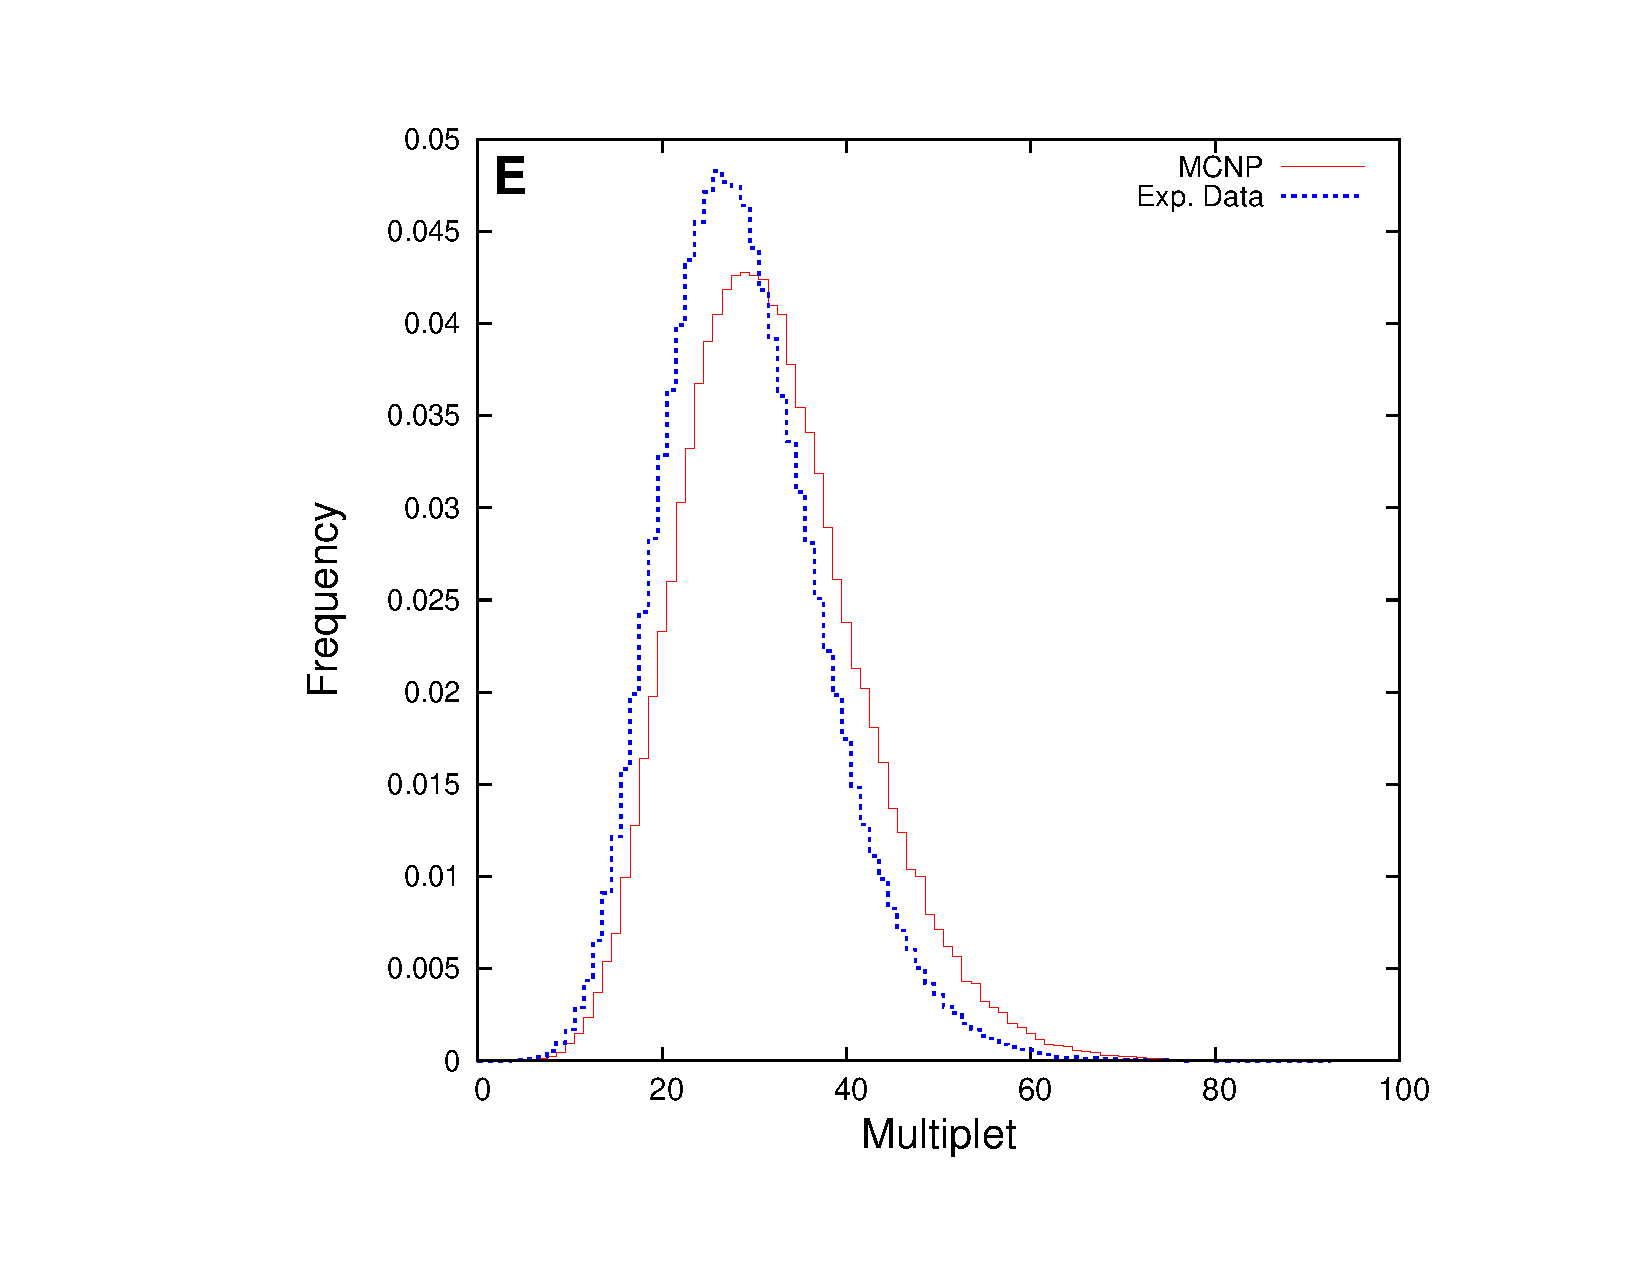
\includegraphics[trim= 1.0in 0.75in 1.0in 0.75in, clip, width=0.5\textwidth]{nubarFigures/trial_1_0_berp_3_0_2000.pdf} &
\hspace{-0.2in}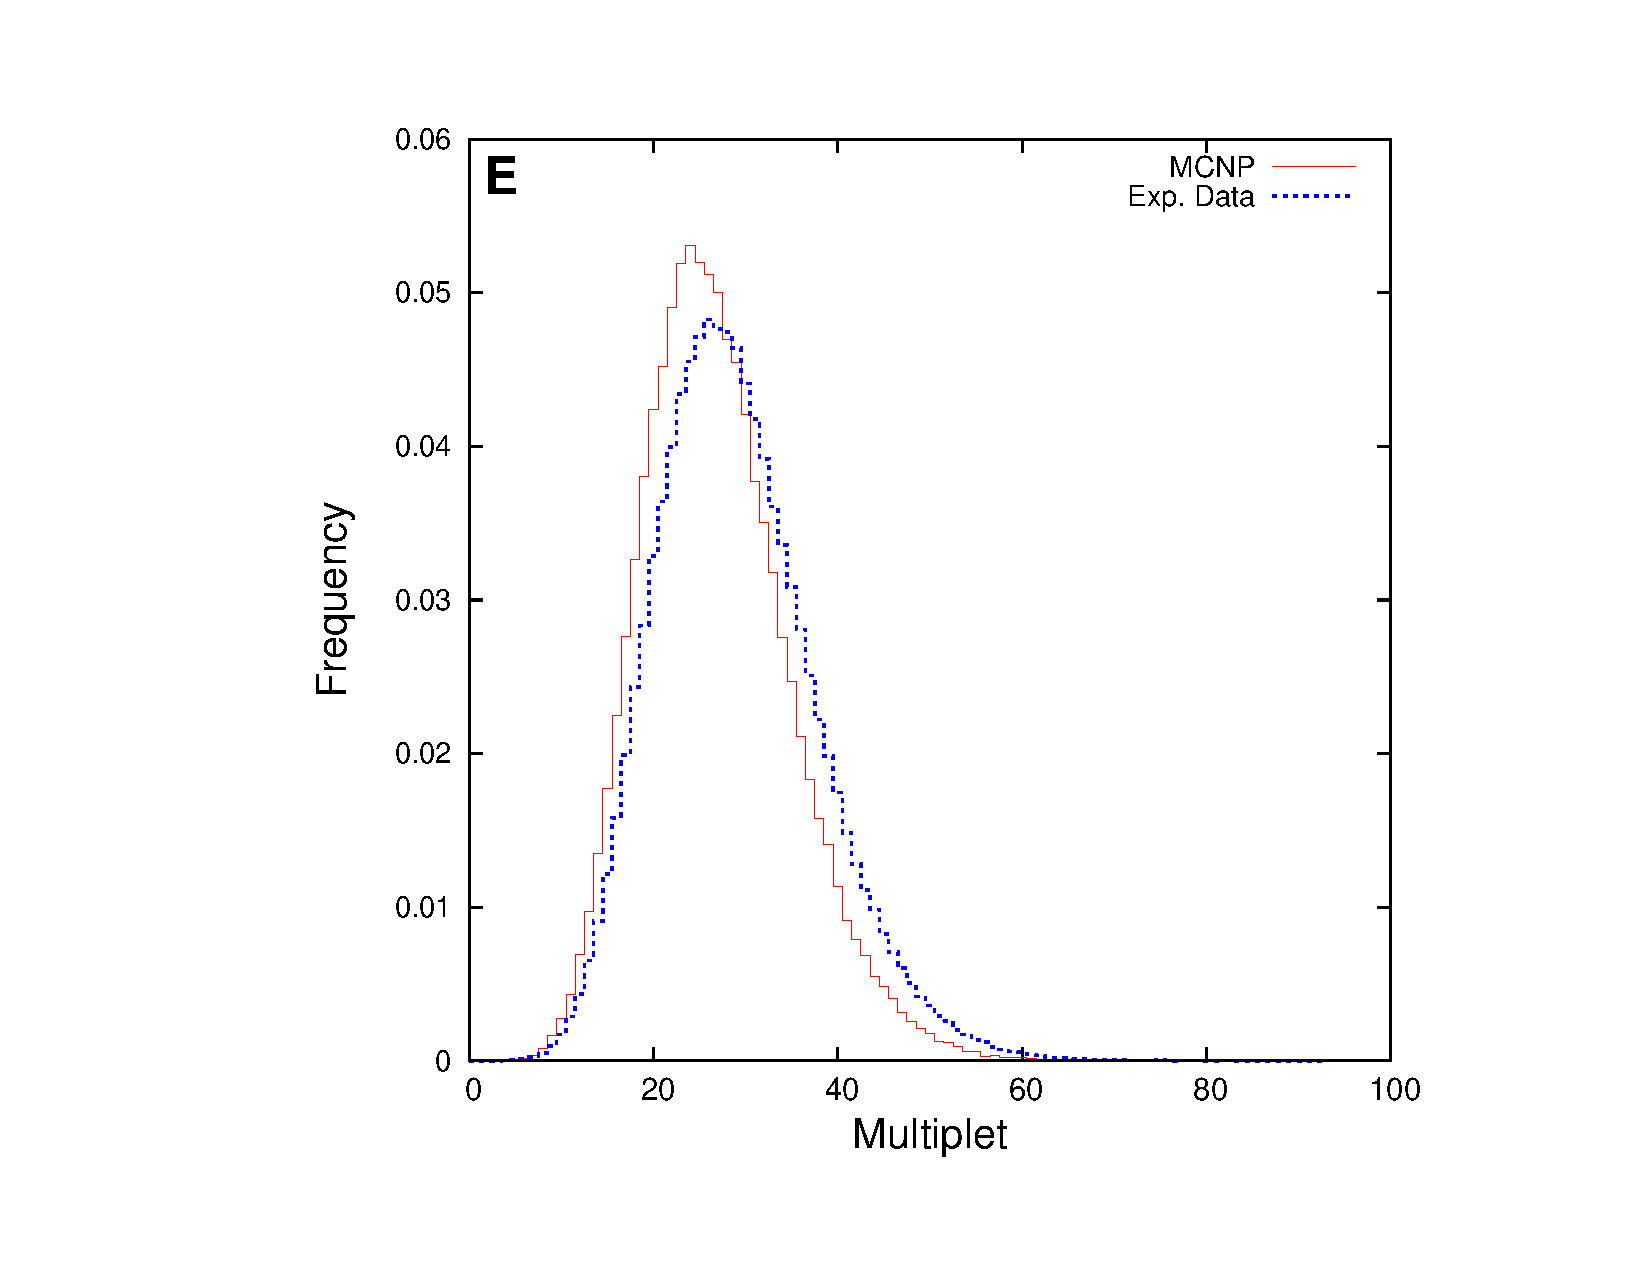
\includegraphics[trim=1.0in 0.75in  1.0in  0.75in, clip, width=0.5\textwidth]{capFigures/trial_0_986_berp_3_0_2000.pdf} \\
\end{array}$
\end{center}
\end{frame}

\begin{frame}
\frametitle{The best \nubar data (trial 303) }
\begin{minipage}{0.49\textwidth}
\begin{figure}[h!]
\centering
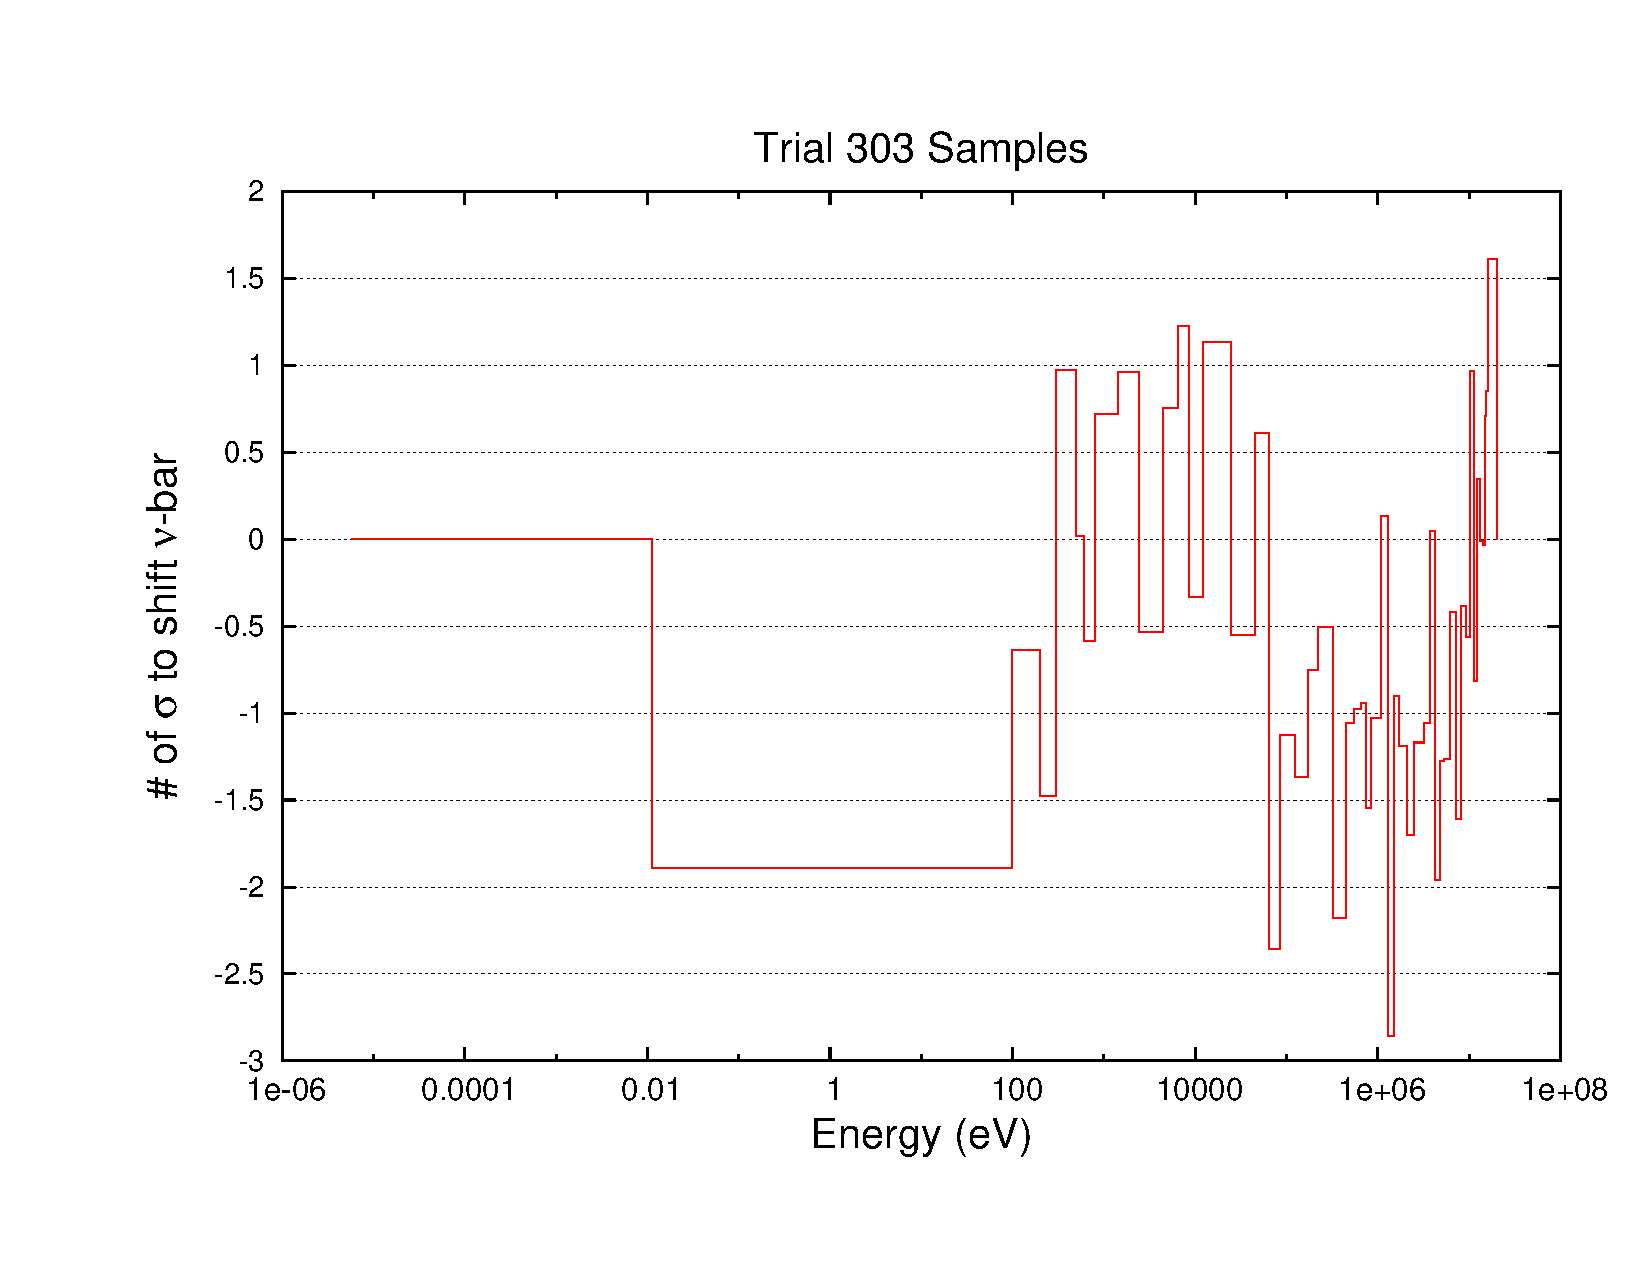
\includegraphics[trim = 0.75in 0.5in 0.25in 0.5in, clip, width=0.99\textwidth]{nubarFigures/nubar_shift.pdf}
\end{figure}
\end{minipage}
\begin{minipage}{0.49\textwidth}
\begin{figure}[h!]
\centering
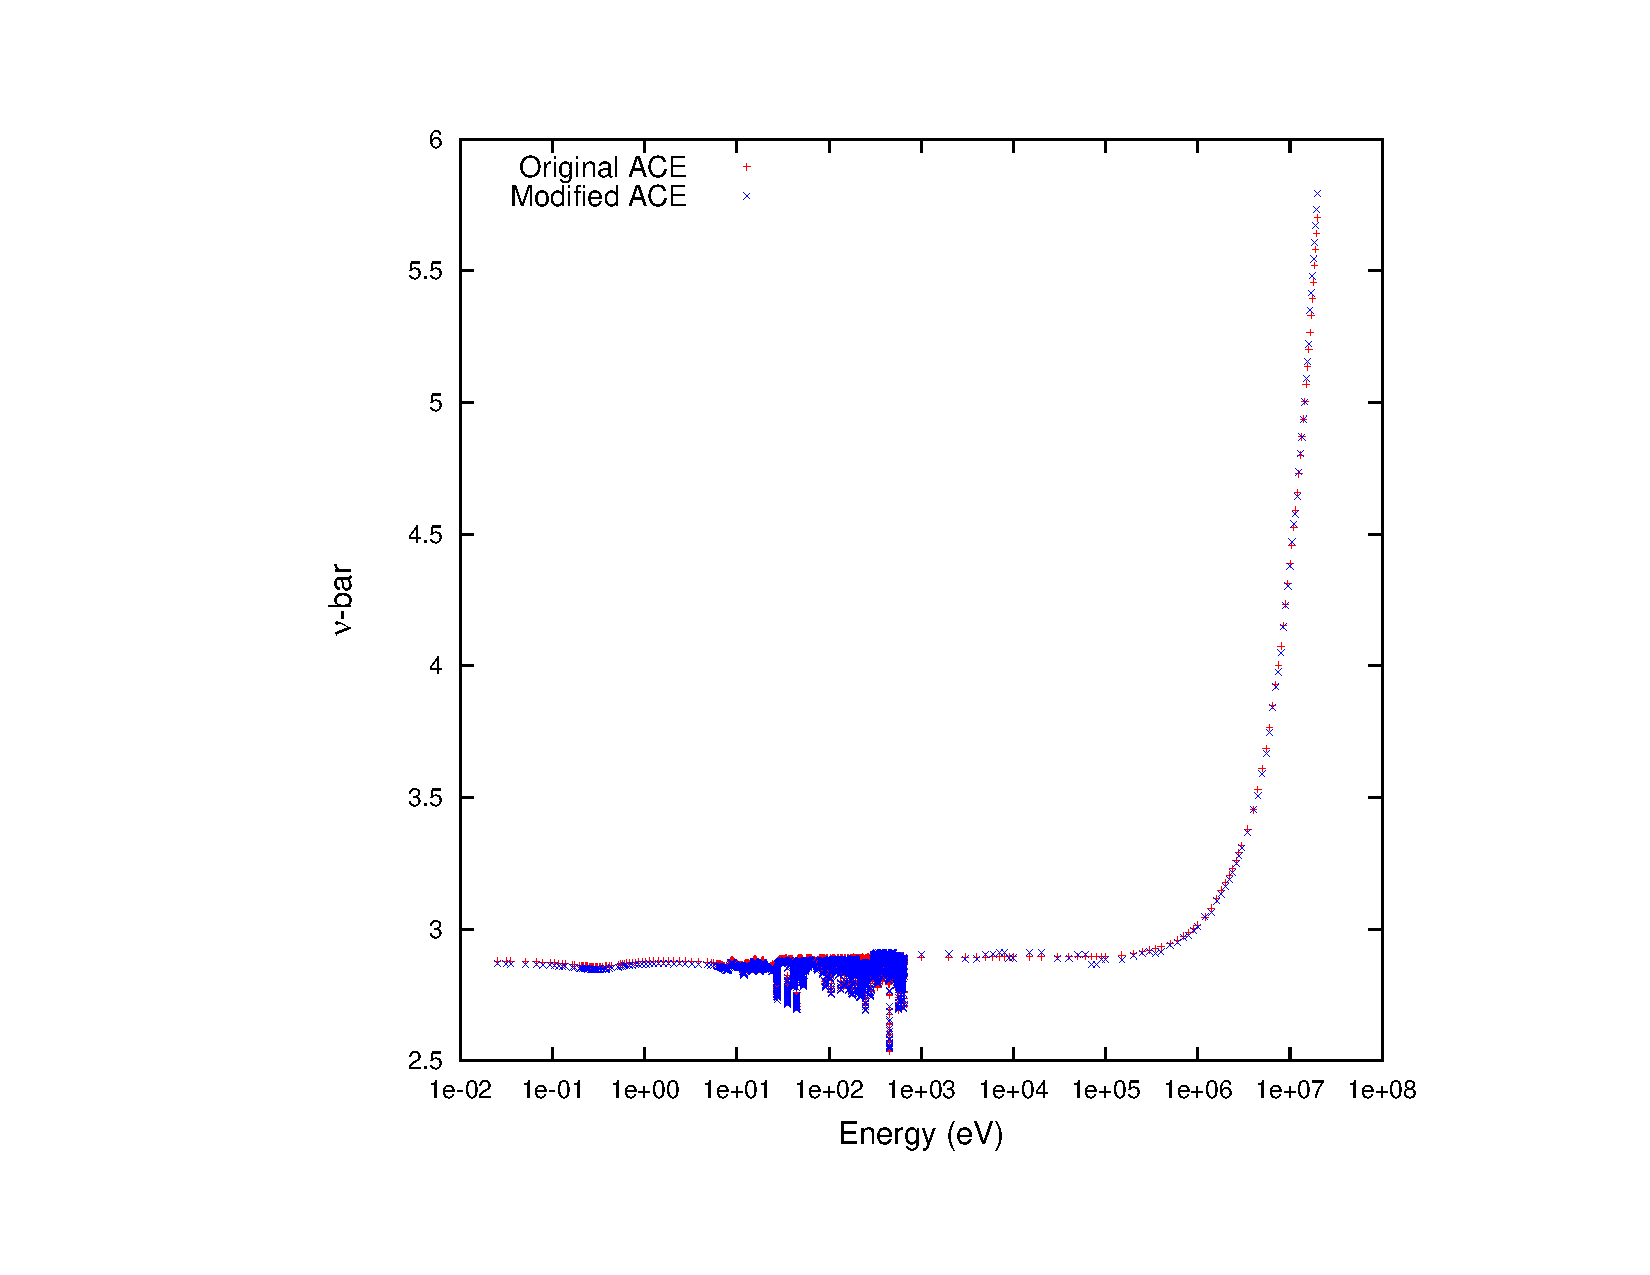
\includegraphics[trim= 1.75in 0.75in 0.75in 0.75in, clip, width=0.99\textwidth]{nubarFigures/nubar.pdf}
\end{figure}
\end{minipage}
\end{frame} 

\begin{frame}
    \frametitle{Fractional shifts to cross sections \\ were made for comparison }
\begin{itemize}
    \item[] Adjusted cross section uniformly at all energies 
        \\ \colG{compensated with $\sigma_{tot}$ or $\sigma_{el}$}
    \item[] Increasing capture cross section was not effective \\
        \colG{relative to variance in data}
    \item[] Scaling fission cross section 1.5\% ($<1 \sigma$) 
        \\ improved multiplicity distributions
        \begin{itemize} \vspace{0.1in}
            \item Adjust elastic scattering ($\sigma_{el}$) to compensate change in $\sigma_f$, for ${E > 1 \text { keV}}$
            \item Better improvement than \emph{uniform} scaling of $\nubar$
        \end{itemize}
\end{itemize} 
\end{frame} 



\setcounter{framenumber}{\value{finalframe}}
\end{document}
